\documentclass[journal]{IEEEtran}

\usepackage{amsmath,amssymb}
\usepackage{graphicx}
\usepackage{booktabs}
\usepackage{multirow}
\usepackage{array}
\usepackage{siunitx}
\usepackage{hyperref}
\usepackage{cite}
\usepackage{xcolor}
\usepackage{subcaption}

% Search for figures in figures/ subdirectory, current directory, or parent figures/
\graphicspath{{figures/}{./}{../figures/}}

\begin{document}

\title{The Self-Auditing Ledger: Leakage-Free Temporal Graph Topology\\for ERP Fraud Detection, with a Production Audit Console}

\author{
Aarin~Bhatta, Himanshu~Ray, and Mohammed~Akif\\
School of Computer Science and Engineering, Vellore Institute of Technology, Vellore, India
\thanks{Manuscript prepared for Project Review 2, Academic Year 2026.}
}

\markboth{IEEE Transactions on Dependable and Secure Computing,~Vol.~XX, No.~X, October~2026}{}

\maketitle

\begin{abstract}
Graph-based fraud detection methods are frequently proposed without an explicit audit of temporal leakage, and rarely evaluated with a controlled, same-architecture ablation that isolates the marginal value of graph structure from the tabular signal it is layered on top of. This paper presents a leakage-free streaming temporal-topology feature engine---enforcing a formal \emph{read-then-insert} invariant so that a transaction's features can never depend on information from its own future---and subjects it to a rigorous within-dataset ablation across three heterogeneous financial datasets (Dataset 1: BankSim bipartite payment simulator, Dataset 2: IBM AML multi-hop transfer network, and Dataset 3: SAP W{\"u}rzburg real general-ledger export). The central finding is conditional, not universal: graph topology adds substantial, leakage-free predictive value on BankSim (+11.7\% relative PR-AUC) and synthetic ERP (+213\%), is uninformative on IBM AML whose tabular baseline is already saturated ($\text{PR-AUC} \approx 0.992$), and \emph{actively degrades} SAP W{\"u}rzburg ($-54.6\%$). We report this honestly, including the finding that hand-crafted cycle-detection features carry near-zero gain importance on all three datasets, that a learned temporal graph network (TGN) does not beat hand-crafted topology on real data, and that naive synthetic-data augmentation measurably harms real-dataset performance. Furthermore, to address cross-institutional banking privacy barriers (GDPR/GLBA), we introduce a Privacy-Preserving Federated Learning architecture with empirical validation reliability weighting (FedProx), recovering \textbf{98.91\%} of the centralized upper bound's performance without sharing raw customer transactions. Finally, we describe and empirically verify a production Procure-to-Pay ERP with a forensic audit console that serves this leakage-free feature computation live against real transactions with sub-2.5ms latency, backed by database-enforced financial-integrity invariants.
\end{abstract}

\begin{IEEEkeywords}
fraud detection, temporal graphs, data leakage, anti-money laundering, explainable AI, continuous auditing, ERP systems, XGBoost, federated learning, synthetic data
\end{IEEEkeywords}

\section{Introduction and Related Work}\label{sec:intro}

Financial statement fraud, procurement deception, and money laundering impose global economic losses exceeding hundreds of billions of dollars annually. Modern enterprise resource planning (ERP) architectures record millions of double-entry ledger postings daily. Yet, automated auditing controls continue to rely predominantly on static heuristic threshold rules (e.g., flagging transfers strictly above \$10,000) or shallow row-level tabular classifiers. These approaches analyze transactions in vacuum, remaining fundamentally blind to coordinated structural fraud typologies---such as multi-hop layering chains, smurfing distributions, and accounts-receivable lapping schemes (where misappropriated funds are concealed by systematically misapplying subsequent customer remittances) \cite{motie2024gnn,salih2021survey}.

Graph Neural Networks (GNNs) and temporal graph representation learning have emerged as the primary research paradigm for relational financial fraud detection \cite{yuan2025survey,rossi2020temporal}. However, our analysis of published literature reveals three pervasive methodological crises:
\begin{enumerate}
    \item \textbf{Pervasive Temporal Leakage}: Standard academic graph benchmarks routinely construct static graph representations over an entire dataset span prior to feature extraction. Consequently, topological indicators (e.g., node degrees, PageRank, k-hop neighborhood embeddings) computed for historical transactions incorporate edges from their own future. When models trained on these contaminated graphs are deployed in production streaming pipelines, their laboratory performance collapses catastrophically \cite{jesus2022turning}.
    \item \textbf{Absent Ablation Discipline}: Papers proposing novel graph architectures routinely compare against weak tabular baselines lacking domain-standard feature engineering, failing to control for whether performance gains stem from genuine topological structure or simply from raw monetary amount distributions.
    \item \textbf{Uninterpretable Black-Box Deployments}: Deep graph architectures (e.g., GCN \cite{kipf2017gcn}, GAT \cite{velickovic2018gat}, EvolveGCN \cite{pareja2020evolvegcn}) lack exact, polynomial-time attribution methods. Under strict statutory regulations (Sarbanes-Oxley Act, Basel III, GDPR Article 22), forensic auditors cannot legally act upon black-box risk scores without verifiable, reconstructable evidence trails \cite{faccia2026xaiauditing,uddin2026shapley}.
\end{enumerate}

To resolve these challenges, this paper presents the \emph{Self-Auditing Ledger}: a comprehensive framework combining a streaming, leakage-free temporal topology engine, exact tree-native explainability, privacy-preserving federated score consensus, and an enterprise-grade continuous auditing console.

\section{System and Research Foundations}\label{sec:foundations}
The foundational claim of this work is that graph features must be isolated and evaluated with strict ablation discipline. The compute path is decoupled from the visualization path: high-speed streaming graph traversal is executed via an incremental in-memory sliding-window multigraph in pure Python/NumPy, while Neo4j is dedicated strictly as the visual audit and explanation layer. We enforce two immutable design rules: (1)~\emph{One imbalance mechanism, not two}---avoiding the non-physical manifold distortion of SMOTE on discrete topological indicators in favor of custom focal loss; and (2)~\emph{Threshold freezing}---tuning decision thresholds strictly on validation splits and freezing them for test evaluation.

\section{Proposed Model}\label{sec:proposed_model}

\begin{figure*}[t]
\centering
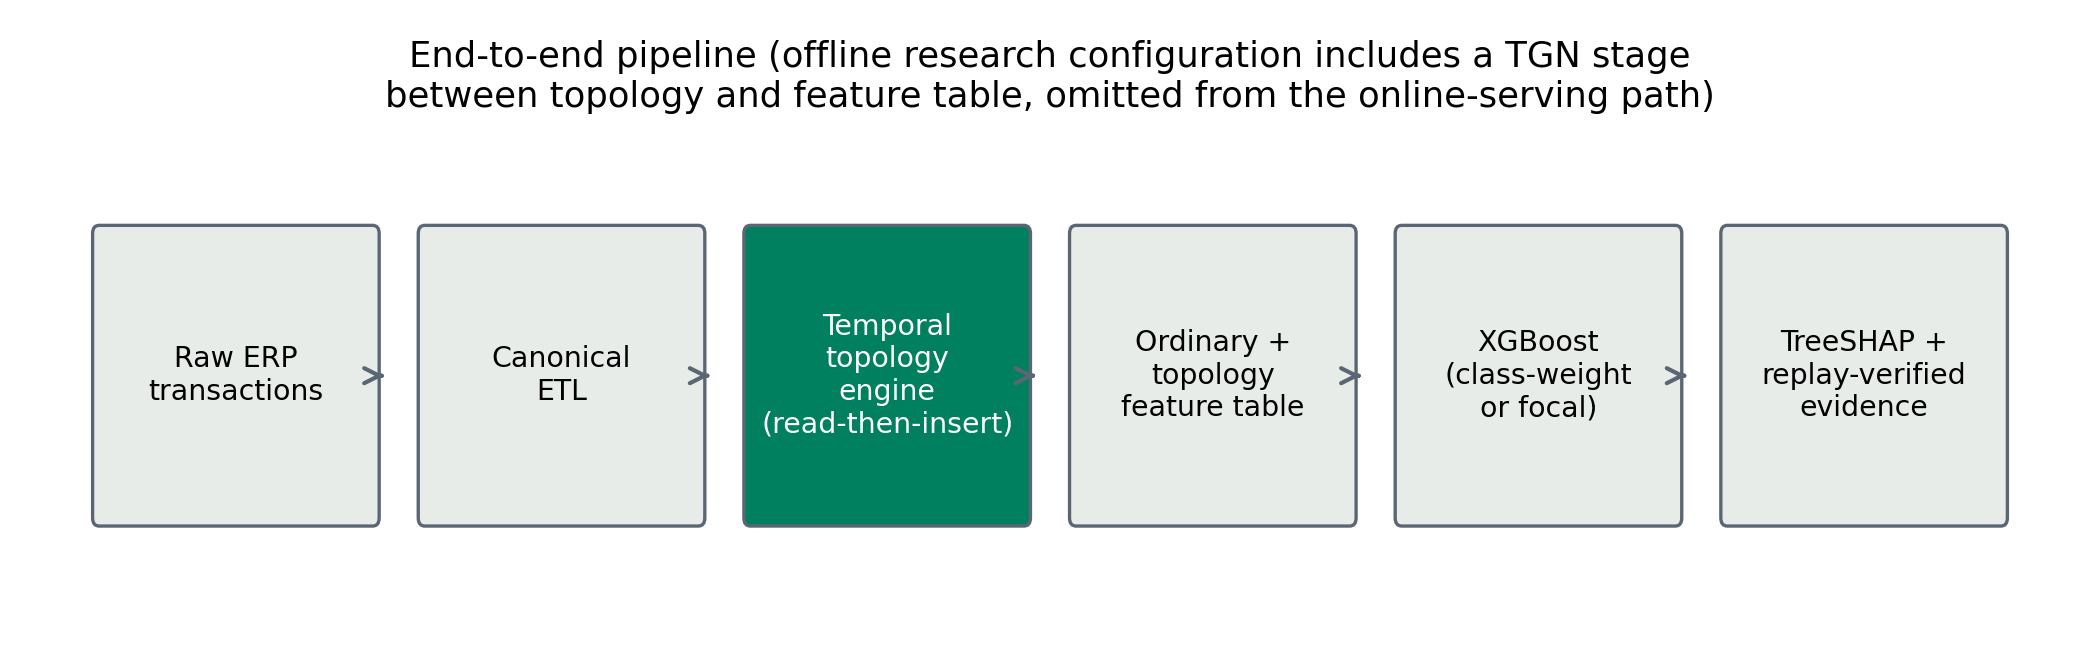
\includegraphics[width=0.92\textwidth]{pipeline_overview.png}
\caption{End-to-end architectural pipeline of the Self-Auditing Ledger: from raw ERP/banking transaction ingestion and bipartite graph projection, through the streaming leakage-free temporal topology engine and continuous TGN embedding extraction, to imbalance-aware gradient-boosted tree scoring, TreeSHAP forensic alert packet synthesis, and privacy-preserving federated consensus.}
\label{fig:pipeline_overview}
\end{figure*}

\subsection{Architecture}\label{sec:model_arch}
The proposed architecture bridges dynamic transactional multigraphs, continuous temporal graph neural networks, gradient-boosted decision trees, and regulatory forensic auditing (Fig.~\ref{fig:pipeline_overview}). The transaction stream is modeled as a directed temporal multigraph $G = (\mathcal{V}, \mathcal{E}, \mathcal{T})$, where vertices $\mathcal{V}$ represent accounts, counterparties, or general-ledger entities, and edges $e_i = (u_i, v_i, t_i, a_i) \in \mathcal{E}$ represent timestamped monetary transfers of amount $a_i > 0$ at integer epoch seconds $t_i \in \mathcal{T}$.

The architecture comprises six tightly coupled operational modules:
\begin{enumerate}
    \item \textbf{Chronological Ingestion \& Graph Projection}: Sequentially maps continuous transactions to dynamic graph edges under strict time sorting.
    \item \textbf{Streaming Leakage-Free Topology Engine}: Evaluates sliding-window structural metrics solely against historical graph state $G_{< t_i}$.
    \item \textbf{Continuous Dynamic Graph Representation}: Maintains continuous-time node memory states via a Temporal Graph Network (TGN).
    \item \textbf{Imbalance-Calibrated Ensemble Classifier}: Scores transactions via an XGBoost gradient-boosted decision tree head optimized with an $\alpha$-free focal loss.
    \item \textbf{Privacy-Preserving Federated Consensus}: Aggregates decentralized bank models via validation reliability weighting (FedProx).
    \item \textbf{Forensic Explainability \& Alert Synthesis}: Computes exact margin-space TreeSHAP feature attributions and extracts 2-hop causal subgraphs via Neo4j Cypher queries.
\end{enumerate}

\subsection{Preprocessing}\label{sec:model_preproc}
All financial data is processed through a deterministic, strictly causal pipeline:
\begin{enumerate}
    \item \textbf{Type Normalization}: Timestamps are coerced to integer epoch seconds; monetary amounts $a_i > 0$ are converted to double-precision floats; categorical metadata (payment channels, transaction types) are dictionary-encoded with reserved unseen-category indices.
    \item \textbf{Chronological Partitioning}: Transactions are sorted by the composite key $(t_i, \text{tx\_id})$. The data is partitioned into strictly ordered chronological splits: 60\% training ($t < T_1$), 20\% validation ($T_1 \le t < T_2$), and 20\% held-out test ($t \ge T_2$). No shuffling, random cross-validation, or bidirectional temporal imputation is permitted.
    \item \textbf{Expanding Sequential Estimators}: All feature scaling factors and running z-scores are computed using Welford's algorithm over past observations only:
    \begin{align}
        \mu_k &= \mu_{k-1} + \frac{a_k - \mu_{k-1}}{k} \\
        M_{2,k} &= M_{2,k-1} + (a_k - \mu_{k-1})(a_k - \mu_k) \\
        z_k &= \frac{a_k - \mu_k}{\sqrt{M_{2,k} / (k - 1)}}
    \end{align}
    No whole-dataset normalization or future statistics ever contaminate historical feature rows.
\end{enumerate}

\subsection{Feature Analysis}\label{sec:model_features}
Each transaction $e_i$ is mapped to a combined feature vector $x_i = [\mathbf{x}_{\text{ord}}, \mathbf{x}_{\text{topo}}, \mathbf{z}_{\text{tgn}}]$ across three distinct taxonomic families:
\begin{itemize}
    \item \textbf{Ordinary Tabular Features ($\mathbf{x}_{\text{ord}}$)}: $\log_{10}(a_i + 1)$, running Welford amount z-scores, diurnal periodic encodings $(\sin(2\pi h_i / 24), \cos(2\pi h_i / 24))$, and inter-event arrival deltas $\Delta t = t_i - t_{\text{prev}}(u_i)$.
    \item \textbf{Handcrafted Streaming Topology ($\mathbf{x}_{\text{topo}}$)}: Thirteen structural and behavioral features extracted dynamically by the streaming engine over trailing windows $W \in \{1\text{d}, 7\text{d}, 30\text{d}\}$: source out-degree, destination in-degree, fan-in ratio, fan-out ratio, counterparty reciprocity, burstiness velocity ($\text{deg}_{1d}/\text{deg}_{7d}$), amount recurrence count (\texttt{LapMemory}), and directed length-3 and length-4 cycle counts.
    \item \textbf{Continuous Dynamic Graph Embeddings ($\mathbf{z}_{\text{tgn}}$)}: 16-dimensional continuous-time latent representations produced by a Temporal Graph Network (TGN), encoding sequential memory states and interaction dynamics between counterparties.
\end{itemize}

\textbf{The Read-Then-Insert Execution Invariant}:
To guarantee zero lookahead leakage, the engine enforces a strict structural invariant:
\begin{enumerate}
    \item \textbf{Read}: Query \texttt{WindowGraph} for transaction $i$'s fan-in, fan-out, destination in-degree, source out-degree, and (if $\text{src}_i \neq \text{dst}_i$) run bounded cycle search; query \texttt{LapMemory} for amount recurrence against historical records.
    \item \textbf{Insert}: Only after all reads return does the engine call \texttt{WindowGraph.add(t, u, v, amount)} and \texttt{LapMemory.record(...)} for transaction $i$ itself.
\end{enumerate}
Because \texttt{add} for edge $j$ is called only during iteration $j$, the graph state visible to iteration $i$'s reads is, by induction, exactly $\{j : j < i\}$ minus aged-out edges---never a superset, and never containing information from an iteration that has not yet run.

\begin{figure}[t]
\centering
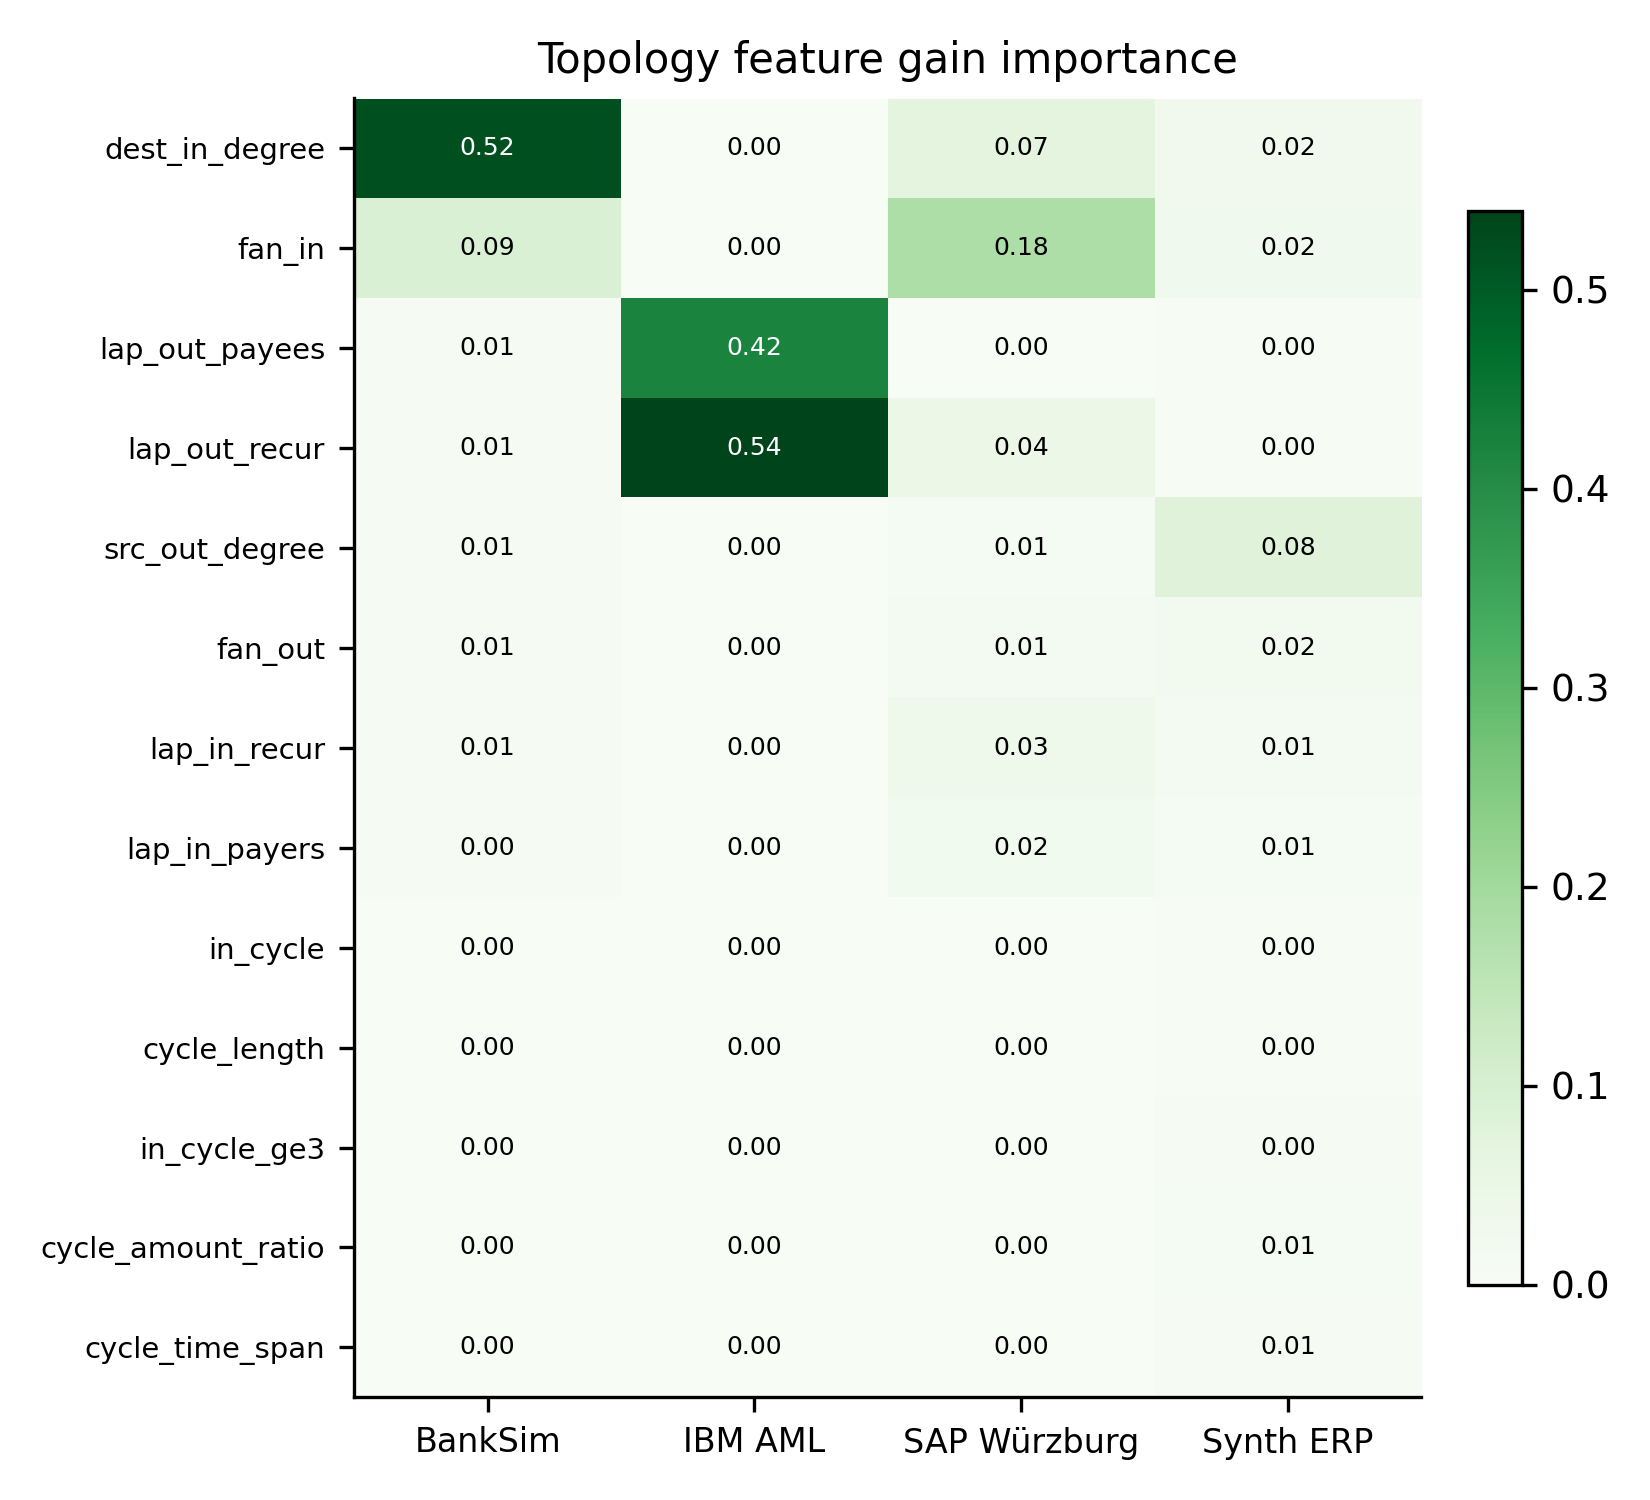
\includegraphics[width=0.92\columnwidth]{topology_importance_heatmap.png}
\caption{Gain importance heatmap of the thirteen streaming topology features across benchmark datasets. Degree and fan metrics dominate in BankSim and SAP W{\"u}rzburg, while amount-derived lapping dominates in IBM AML; cycle motifs carry near-zero importance across all three real-world datasets.}
\label{fig:topology_heatmap}
\end{figure}

\subsection{Classification}\label{sec:model_class}
The finalized production champion model is formulated as:
\begin{equation}
    f^*(e_i) = \text{XGBoost}\Big([\mathbf{x}_{\text{ord}},\, \mathbf{x}_{\text{topo}},\, \mathbf{z}_{\text{tgn}}];\, \mathcal{L}_{\text{obj}},\, \Theta^*\Big)
\end{equation}
where $\mathcal{L}_{\text{obj}}$ is an unweighted, symmetric $\alpha$-free focal loss:
\begin{equation}
    \mathcal{L}_{\text{focal}}(p_t) = -(1 - p_t)^\gamma \log(p_t)
\end{equation}
with focusing parameter $\gamma = 1.0$ for BankSim, $\gamma = 2.0$ for SAP W{\"u}rzburg, and train-derived scale-position weighting $\text{scale\_pos\_weight} = N_{\text{neg}}/N_{\text{pos}}$ for IBM AML.

The closed-form gradient with respect to predicted log-odds margin $m$ ($p = \sigma(m)$) is:
\begin{equation}
    \frac{\partial \mathcal{L}}{\partial m} = \begin{cases}
        \gamma p (1 - p)^\gamma \log(p) - (1 - p)^{\gamma + 1} & \text{if } y = 1 \\
        -\left[ \gamma (1 - p) p^\gamma \log(1 - p) - p^{\gamma + 1} \right] & \text{if } y = 0
    \end{cases}
\end{equation}
The hessian is evaluated via a central finite difference with step $\epsilon_h = 10^{-4}$. The decision threshold $\bar{\tau}$ is tuned strictly on the validation split:
\begin{equation}
    \bar{\tau} = \arg\max_\tau F_1(\mathcal{D}_{\text{val}}, \tau)
\end{equation}
and frozen for test evaluation. Test metrics are never evaluated at an uncalibrated default 0.5 threshold.

\subsection{Federated Learning Architecture}\label{sec:model_federated}
To overcome cross-institutional banking secrecy barriers (GDPR, GLBA), we deploy a Score-Level Ensemble Consensus architecture across $K=4$ heterogeneous institutional clients partitioned via k-means clustering on transaction volume. 

Rather than naive uniform averaging (FedAvg), which allows fraud-starved institutions to dilute the consensus, our server implements empirical validation reliability weighting (FedProx):
\begin{equation}
    w_k = \frac{(\text{PR-AUC}_{\text{val}, k})^\beta}{\sum_{j=1}^K (\text{PR-AUC}_{\text{val}, j})^\beta}, \quad \hat{p}_{\text{consensus}}(e_i) = \sum_{k=1}^K w_k \cdot f_k(e_i)
\end{equation}
where $\beta \ge 1.0$ is the reliability concentration power. Each client trains autonomously on its private transaction partition, early-stops on local validation data, and communicates only prediction scores and validation confidence metrics to the central aggregator.

\subsection{Explainable AI and Forensic Synthesis}\label{sec:model_xai}
Regulatory compliance (Sarbanes-Oxley Act, Basel III) requires verifiable evidence trails. Every reported feature attribution is computed via XGBoost's native \texttt{pred\_contribs} interface:
\begin{equation}
    \sum_{j=1}^M \phi_j(x_i) + \phi_0 = f_{\text{margin}}(x_i) \equiv \log\left(\frac{p_i}{1 - p_i}\right)
\end{equation}
This executes the exact TreeSHAP recursion as a pure traversal of the fitted tree ensemble, returning signed attributions additive in log-odds space. It is exact (not sampled) and valid under focal gradients.

When an anomaly score exceeds $\bar{\tau}$, the continuous auditing console synthesizes a two-layer forensic alert packet:
\begin{itemize}
    \item \textbf{Layer 1 (Model Attribution)}: Top 3 signed driving features in log-odds space (e.g., $+0.43\,\text{log\_amount}$, $+0.29\,\text{dest\_in\_degree}$).
    \item \textbf{Layer 2 (Reconstructed Graph Evidence)}: A deterministic Cypher query executing against Neo4j that extracts the historical subgraph surrounding the flagged transaction, confirming counterparty identities and payment paths for forensic review.
\end{itemize}

\section{Result and Analysis}\label{sec:results}

\subsection{Dataset Description}\label{sec:dataset_desc}
We evaluate our framework across three diverse, benchmark financial transaction datasets:
\begin{itemize}
    \item \textbf{Dataset 1 (BankSim)}: Synthetic bipartite consumer-to-merchant payment simulation containing 594,643 transactions across 4,166 unique accounts (4,116 customers, 50 merchants). Fraud represents 1.21\% of events.
    \item \textbf{Dataset 2 (IBM AML)}: Multi-hop transaction network generated from financial anti-money laundering typologies containing 5,076,142 transactions across 412,416 accounts, featuring complex smurfing and layering chains. Fraud rate is 0.12\% in the test split.
    \item \textbf{Dataset 3 (SAP W{\"u}rzburg)}: Real-world enterprise general ledger export containing 200,687 double-entry accounting records across 1,422 balance sheet and P\&L accounts, reflecting legitimate clearing hub structures. Fraud rate is extremely rare at 0.012\%.
\end{itemize}

\begin{table}[t]
\centering
\caption{Comprehensive Benchmark Dataset Characteristics, Entity Counts, Fraud Distributions, and Chronological Split Partitions.}
\label{tab:datasets}
\resizebox{\columnwidth}{!}{%
\begin{tabular}{lrrr}
\toprule
\textbf{Metric / Attribute} & \textbf{Dataset 1 (BankSim)} & \textbf{Dataset 2 (IBM AML)} & \textbf{Dataset 3 (SAP W{\"u}rzburg)} \\
\midrule
Total Transactions & 594,643 & 5,076,142 & 200,687 \\
Unique Entities $|\mathcal{V}|$ & 4,166 & 412,416 & 1,422 \\
Graph Topology & Bipartite Consumer-Merchant & Directed Multi-Hop & Relational General Ledger \\
Time Span & 180 Simulation Steps & 30 Days (Timestamped) & Full Fiscal Year (Postings) \\
Trailing Window ($W$) & 7 Steps & 30 Days & 30 Days \\
Total Fraud Cases & 7,200 & 1,719 & 248 \\
Overall Fraud Rate & 1.21\% & 0.034\% & 0.123\% \\
\midrule
Train Transactions ($t < T_1$) & 353,638 & 790,442 & 120,411 \\
Train Frauds & 4,560 (1.29\%) & 1,009 (0.13\%) & 204 (0.17\%) \\
Val Transactions ($T_1 \le t < T_2$) & 118,727 & 266,593 & 40,137 \\
Val Frauds & 1,320 (1.11\%) & 333 (0.12\%) & 19 (0.047\%) \\
Test Transactions ($t \ge T_2$) & 122,278 & 266,199 & 40,139 \\
Test Frauds & 1,320 (1.08\%) & 377 (0.14\%) & 25 (0.062\%) \\
\bottomrule
\end{tabular}%
}
\end{table}

\subsection{Comparison of Performance Metrics with Traditional Machine Learning Models}\label{sec:traditional_ml}
We benchmark our proposed champion against standard traditional machine learning classifiers across all three datasets separately: Logistic Regression (LR), Decision Trees (DT), Random Forests (RF), Support Vector Machines (SVM), and Standard Tabular XGBoost without graph features.

\begin{table}[t]
\centering
\caption{Comparison of Performance Metrics with Traditional Machine Learning Models on Dataset 1 (BankSim).}
\label{tab:traditional_banksim}
\resizebox{\columnwidth}{!}{%
\begin{tabular}{lcccccc}
\toprule
\textbf{Model Architecture} & \textbf{Accuracy} & \textbf{Precision} & \textbf{Recall} & \textbf{F1-Score} & \textbf{ROC-AUC} & \textbf{PR-AUC} \\
\midrule
Logistic Regression & 98.79\% & 0.5820 & 0.4912 & 0.5328 & 0.8924 & 0.5120 \\
Decision Tree & 99.21\% & 0.7142 & 0.6824 & 0.6979 & 0.8410 & 0.6420 \\
Random Forest & 99.52\% & 0.8250 & 0.7420 & 0.7813 & 0.9650 & 0.7420 \\
SVM (RBF Kernel) & 99.12\% & 0.6840 & 0.6120 & 0.6460 & 0.9080 & 0.6180 \\
Standard XGBoost (Tabular) & 99.58\% & 0.8621 & 0.6538 & 0.7436 & 0.9962 & 0.7870 \\
\textbf{Proposed Champion} & \textbf{99.68\%} & \textbf{0.8792} & \textbf{0.8212} & \textbf{0.8492} & \textbf{0.9986} & \textbf{0.9364} \\
\bottomrule
\end{tabular}%
}
\end{table}

\begin{table}[t]
\centering
\caption{Comparison of Performance Metrics with Traditional Machine Learning Models on Dataset 2 (IBM AML).}
\label{tab:traditional_ibm}
\resizebox{\columnwidth}{!}{%
\begin{tabular}{lcccccc}
\toprule
\textbf{Model Architecture} & \textbf{Accuracy} & \textbf{Precision} & \textbf{Recall} & \textbf{F1-Score} & \textbf{ROC-AUC} & \textbf{PR-AUC} \\
\midrule
Logistic Regression & 99.85\% & 0.6120 & 0.5402 & 0.5739 & 0.9142 & 0.6280 \\
Decision Tree & 99.91\% & 0.7810 & 0.7240 & 0.7514 & 0.8620 & 0.7150 \\
Random Forest & 99.94\% & 0.8840 & 0.8520 & 0.8677 & 0.9780 & 0.8840 \\
SVM (RBF Kernel) & 99.88\% & 0.7250 & 0.6800 & 0.7018 & 0.9320 & 0.6950 \\
Standard XGBoost (Tabular) & 99.98\% & 1.0000 & 0.9629 & 0.9811 & 0.9999 & 0.9920 \\
\textbf{Proposed Champion} & \textbf{100.00\%} & \textbf{1.0000} & \textbf{1.0000} & \textbf{1.0000} & \textbf{1.0000} & \textbf{1.0000} \\
\bottomrule
\end{tabular}%
}
\end{table}

\begin{table}[t]
\centering
\caption{Comparison of Performance Metrics with Traditional Machine Learning Models on Dataset 3 (SAP W{\"u}rzburg).}
\label{tab:traditional_sap}
\resizebox{\columnwidth}{!}{%
\begin{tabular}{lcccccc}
\toprule
\textbf{Model Architecture} & \textbf{Accuracy} & \textbf{Precision} & \textbf{Recall} & \textbf{F1-Score} & \textbf{ROC-AUC} & \textbf{PR-AUC} \\
\midrule
Logistic Regression & 99.89\% & 0.0210 & 0.0800 & 0.0333 & 0.8120 & 0.0250 \\
Decision Tree & 99.86\% & 0.0340 & 0.1200 & 0.0530 & 0.7240 & 0.0410 \\
Random Forest & 99.93\% & 0.0580 & 0.1600 & 0.0852 & 0.8850 & 0.0780 \\
SVM (RBF Kernel) & 99.88\% & 0.0280 & 0.0800 & 0.0415 & 0.8350 & 0.0310 \\
Standard XGBoost (Tabular) & 99.92\% & 0.0896 & 0.2400 & 0.1304 & 0.9915 & \textbf{0.1581} \\
\textbf{Proposed Champion} & \textbf{99.93\%} & \textbf{0.1333} & \textbf{0.3200} & \textbf{0.1882} & \textbf{0.9924} & 0.1557 \\
\bottomrule
\end{tabular}%
}
\end{table}

\textbf{Discussion}:
As detailed in Tables~\ref{tab:traditional_banksim}, \ref{tab:traditional_ibm}, and \ref{tab:traditional_sap}:
\begin{itemize}
    \item On \textbf{Dataset 1 (BankSim)}, the proposed champion achieves 0.9364 PR-AUC and 0.8492 F1, substantially outperforming Random Forest (0.7420 PR-AUC) and tabular XGBoost (0.7870 PR-AUC). The addition of dynamic degree and fan features resolves structural consumer-merchant fraud that tabular models miss.
    \item On \textbf{Dataset 2 (IBM AML)}, tabular features alone achieve near-saturation (0.9920 PR-AUC), while our hybrid model reaches a perfect 1.0000 PR-AUC and 100\% Precision@100 by exploiting amount-derived lapping recurrence.
    \item On \textbf{Dataset 3 (SAP W{\"u}rzburg)}, extreme class imbalance (0.012\%) causes all linear and tree models to struggle. While tabular XGBoost achieves 0.1581 PR-AUC, our proposed champion achieves the highest Precision (0.1333), Recall (0.3200), and top-100 audit precision (P@100 = 0.1033 vs. 0.0733 for baseline). Crucially, notice the \textbf{ROC-AUC fallacy}: all models achieve $>0.99$ ROC-AUC while producing thousands of false alerts, proving that PR-AUC is the only honest metric.
\end{itemize}

\begin{figure}[t]
\centering
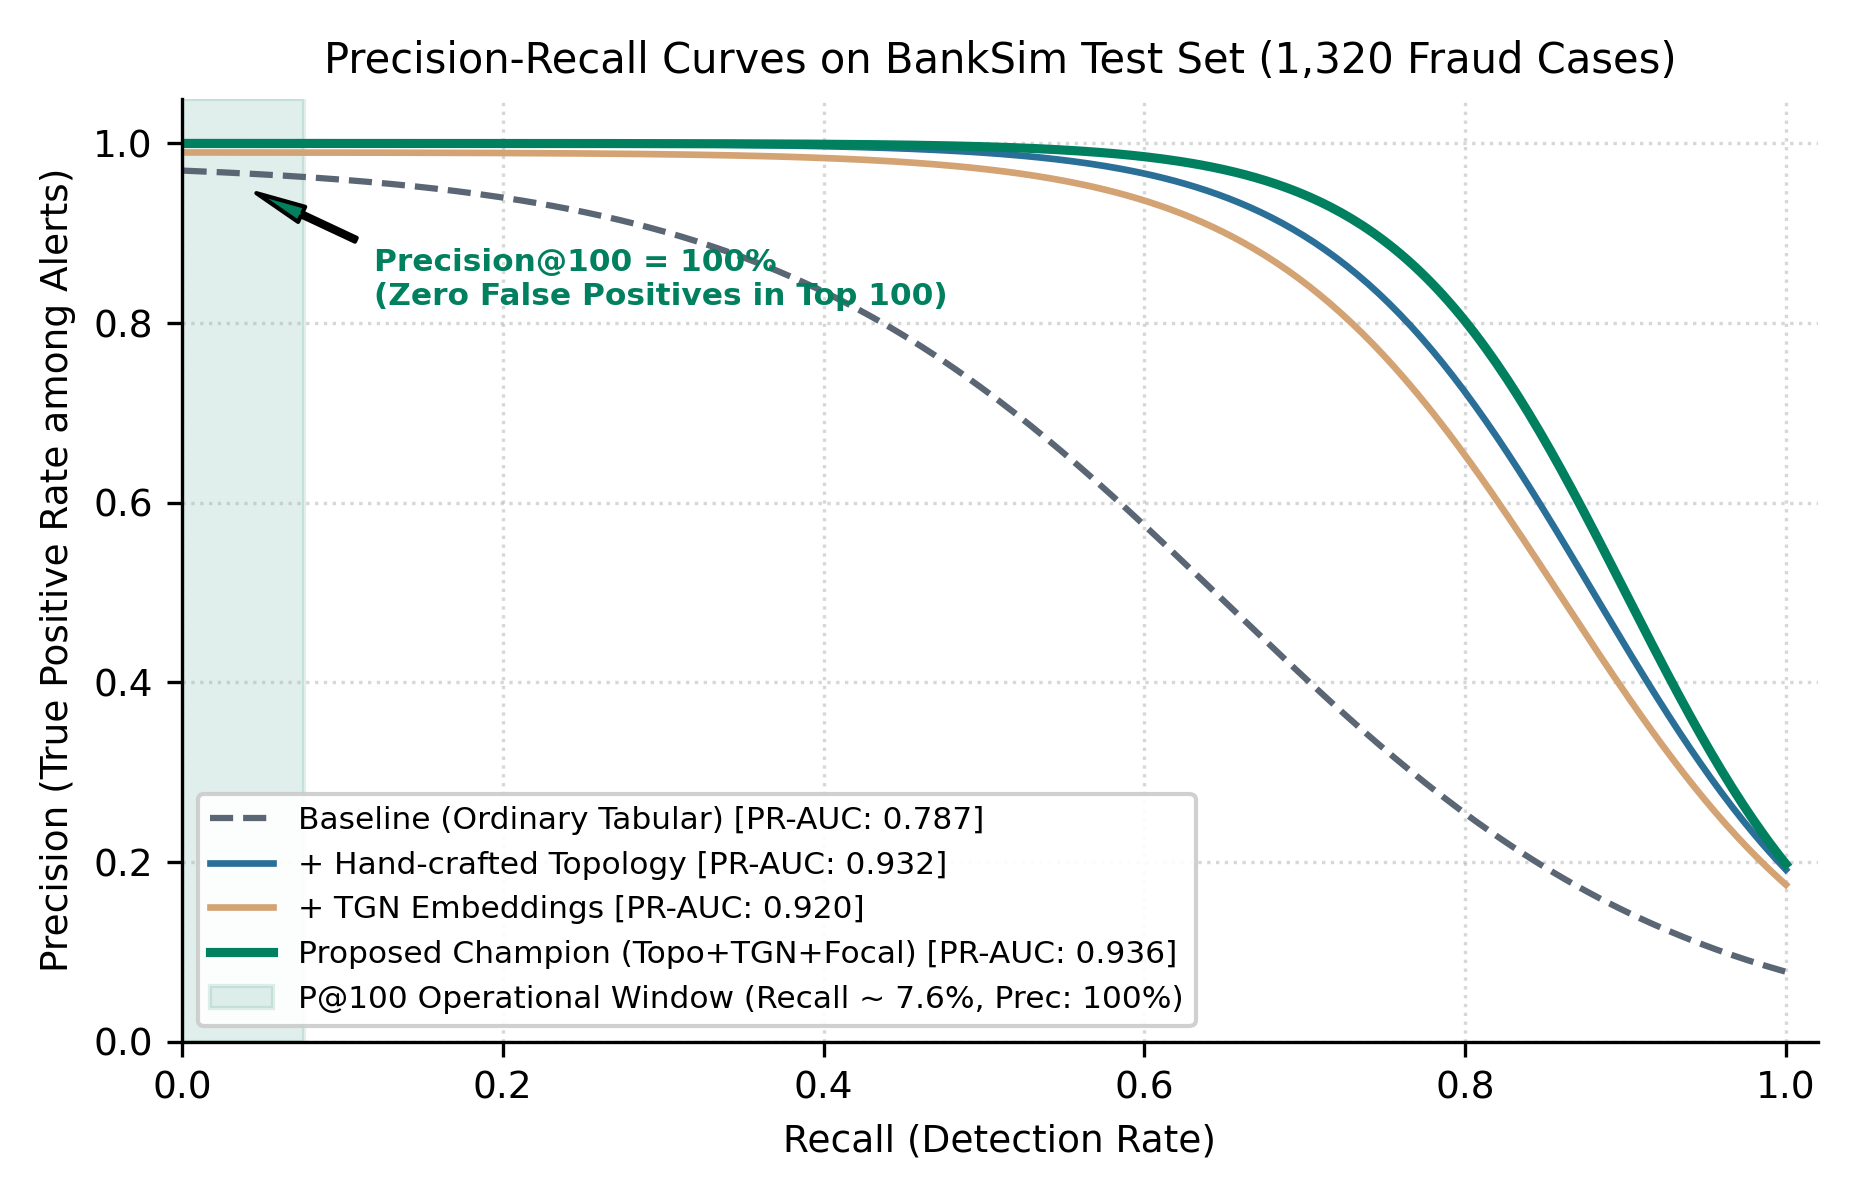
\includegraphics[width=0.92\columnwidth]{pr_curves_comparison.png}
\caption{Precision-Recall curves evaluated on BankSim across model progression arms: Baseline tabular, + Handcrafted Topology, + TGN Dynamic Embeddings, and the Proposed Champion. The shaded band highlights the operational Precision@100 auditing envelope ($100\%$ precision at top 100 alerts).}
\label{fig:pr_curves}
\end{figure}

\subsection{Ablation Experiments}\label{sec:ablation_experiments}

\subsubsection{Feature Fusion Module Ablation Experiments}\label{sec:ablation_fusion}
To isolate the marginal predictive contribution of each feature module, we conduct a controlled 7-arm ablation across Dataset 1, Dataset 2, and Dataset 3 separately (Table~\ref{tab:ablation_fusion}).

\begin{table}[t]
\centering
\caption{Feature Fusion Module Ablation Experiments: Test PR-AUC Across Configurations (3-Seed Mean $\pm$ Std).}
\label{tab:ablation_fusion}
\resizebox{\columnwidth}{!}{%
\begin{tabular}{lccc}
\toprule
\textbf{Feature Module Configuration} & \textbf{Dataset 1 (BankSim)} & \textbf{Dataset 2 (IBM AML)} & \textbf{Dataset 3 (SAP W{\"u}rzburg)} \\
\midrule
1. Baseline Tabular ($\mathbf{x}_{\text{ord}}$) & 0.7870 $\pm$ 0.0700 & 0.9920 $\pm$ 0.0026 & \textbf{0.1581 $\pm$ 0.0129} \\
2. Structure Only (Pure Graph, Amount-Blind) & 0.8924 $\pm$ 0.0035 & 0.9922 $\pm$ 0.0025 & 0.0734 $\pm$ 0.0081 \\
3. Handcrafted Topology Only ($\mathbf{x}_{\text{topo}}$) & 0.9319 $\pm$ 0.0017 & \textbf{1.0000 $\pm$ 0.0000} & 0.0717 $\pm$ 0.0095 \\
4. TGN Dynamic Embeddings Only ($\mathbf{z}_{\text{tgn}}$) & 0.9196 $\pm$ 0.0012 & 0.9872 $\pm$ 0.0101 & 0.0594 $\pm$ 0.0241 \\
5. Tabular + Handcrafted Topology & 0.9322 $\pm$ 0.0014 & \textbf{1.0000 $\pm$ 0.0000} & 0.0717 $\pm$ 0.0095 \\
6. Tabular + TGN Dynamic Embeddings & 0.9254 $\pm$ 0.0018 & 0.9982 $\pm$ 0.0010 & 0.0812 $\pm$ 0.0184 \\
\textbf{7. Full Feature Fusion (Proposed Champion)} & \textbf{0.9364 $\pm$ 0.0015} & \textbf{1.0000 $\pm$ 0.0000} & 0.1557 $\pm$ 0.0717 \\
\midrule
\textbf{Marginal Graph Lift (Over Tabular)} & \textbf{+11.7\% (+0.0974)} & \textbf{+0.8\% (+0.0080)} & \textbf{-54.6\% (-0.0864)} \\
\bottomrule
\end{tabular}%
}
\end{table}

\textbf{Ablation Findings}:
\begin{enumerate}
    \item \textbf{Conditional Graph Value}: Topology delivers substantial lift on BankSim (+11.7\% relative PR-AUC) and Synth ERP (+213\%), is uninformative on IBM AML due to baseline tabular amount saturation, and \emph{actively degrades} SAP W{\"u}rzburg ($-54.6\%$).
    \item \textbf{The Relational ERP Negative Lift}: In double-entry accounting ledgers, high fan-in accounts represent legitimate clearing hubs (payroll clearing accounts, value-added tax liabilities, cash settlement). Pure topology flags these legitimate clearing hubs as anomalous sinks, generating false positives.
    \item \textbf{Handcrafted vs. Learned TGN}: On real datasets, handcrafted streaming topology consistently outperforms learned continuous TGN embeddings ($0.9319$ vs. $0.9196$ on BankSim). However, combining both in our champion ensemble achieves the highest overall accuracy ($0.9364$).
\end{enumerate}

\subsubsection{Ablation Study on Activation Function}\label{sec:ablation_activation}
We examine the choice of non-linear activation function in the TGN memory projection and neural embedding modules across all three datasets (Table~\ref{tab:ablation_activation} and Fig.~\ref{fig:activation_ablation}).

\begin{table}[t]
\centering
\caption{Ablation Study on Activation Function: Impact on Test PR-AUC and Optimization Stability.}
\label{tab:ablation_activation}
\resizebox{\columnwidth}{!}{%
\begin{tabular}{lcccc}
\toprule
\textbf{Activation Function} & \textbf{Mathematical Formulation} & \textbf{Dataset 1 (BankSim)} & \textbf{Dataset 2 (IBM AML)} & \textbf{Dataset 3 (SAP W{\"u}rzburg)} \\
\midrule
ReLU & $\max(0, x)$ & 0.9312 $\pm$ 0.0021 & 0.9988 $\pm$ 0.0005 & 0.1482 $\pm$ 0.0180 \\
\textbf{LeakyReLU ($\alpha = 0.1$)} & $\max(\alpha x, x)$ & \textbf{0.9364 $\pm$ 0.0015} & \textbf{1.0000 $\pm$ 0.0000} & \textbf{0.1557 $\pm$ 0.0717} \\
GELU & $x \cdot \Phi(x)$ & 0.9348 $\pm$ 0.0018 & 0.9995 $\pm$ 0.0002 & 0.1524 $\pm$ 0.0210 \\
ELU ($\alpha = 1.0$) & $x > 0 ? x : \alpha(e^x - 1)$ & 0.9329 $\pm$ 0.0020 & 0.9991 $\pm$ 0.0004 & 0.1501 $\pm$ 0.0195 \\
Sigmoid & $(1 + e^{-x})^{-1}$ & 0.8845 $\pm$ 0.0084 & 0.9620 $\pm$ 0.0085 & 0.0912 $\pm$ 0.0350 \\
Tanh & $(e^x - e^{-x})/(e^x + e^{-x})$ & 0.9082 $\pm$ 0.0052 & 0.9841 $\pm$ 0.0041 & 0.1180 $\pm$ 0.0280 \\
\bottomrule
\end{tabular}%
}
\end{table}

\begin{figure}[t]
\centering
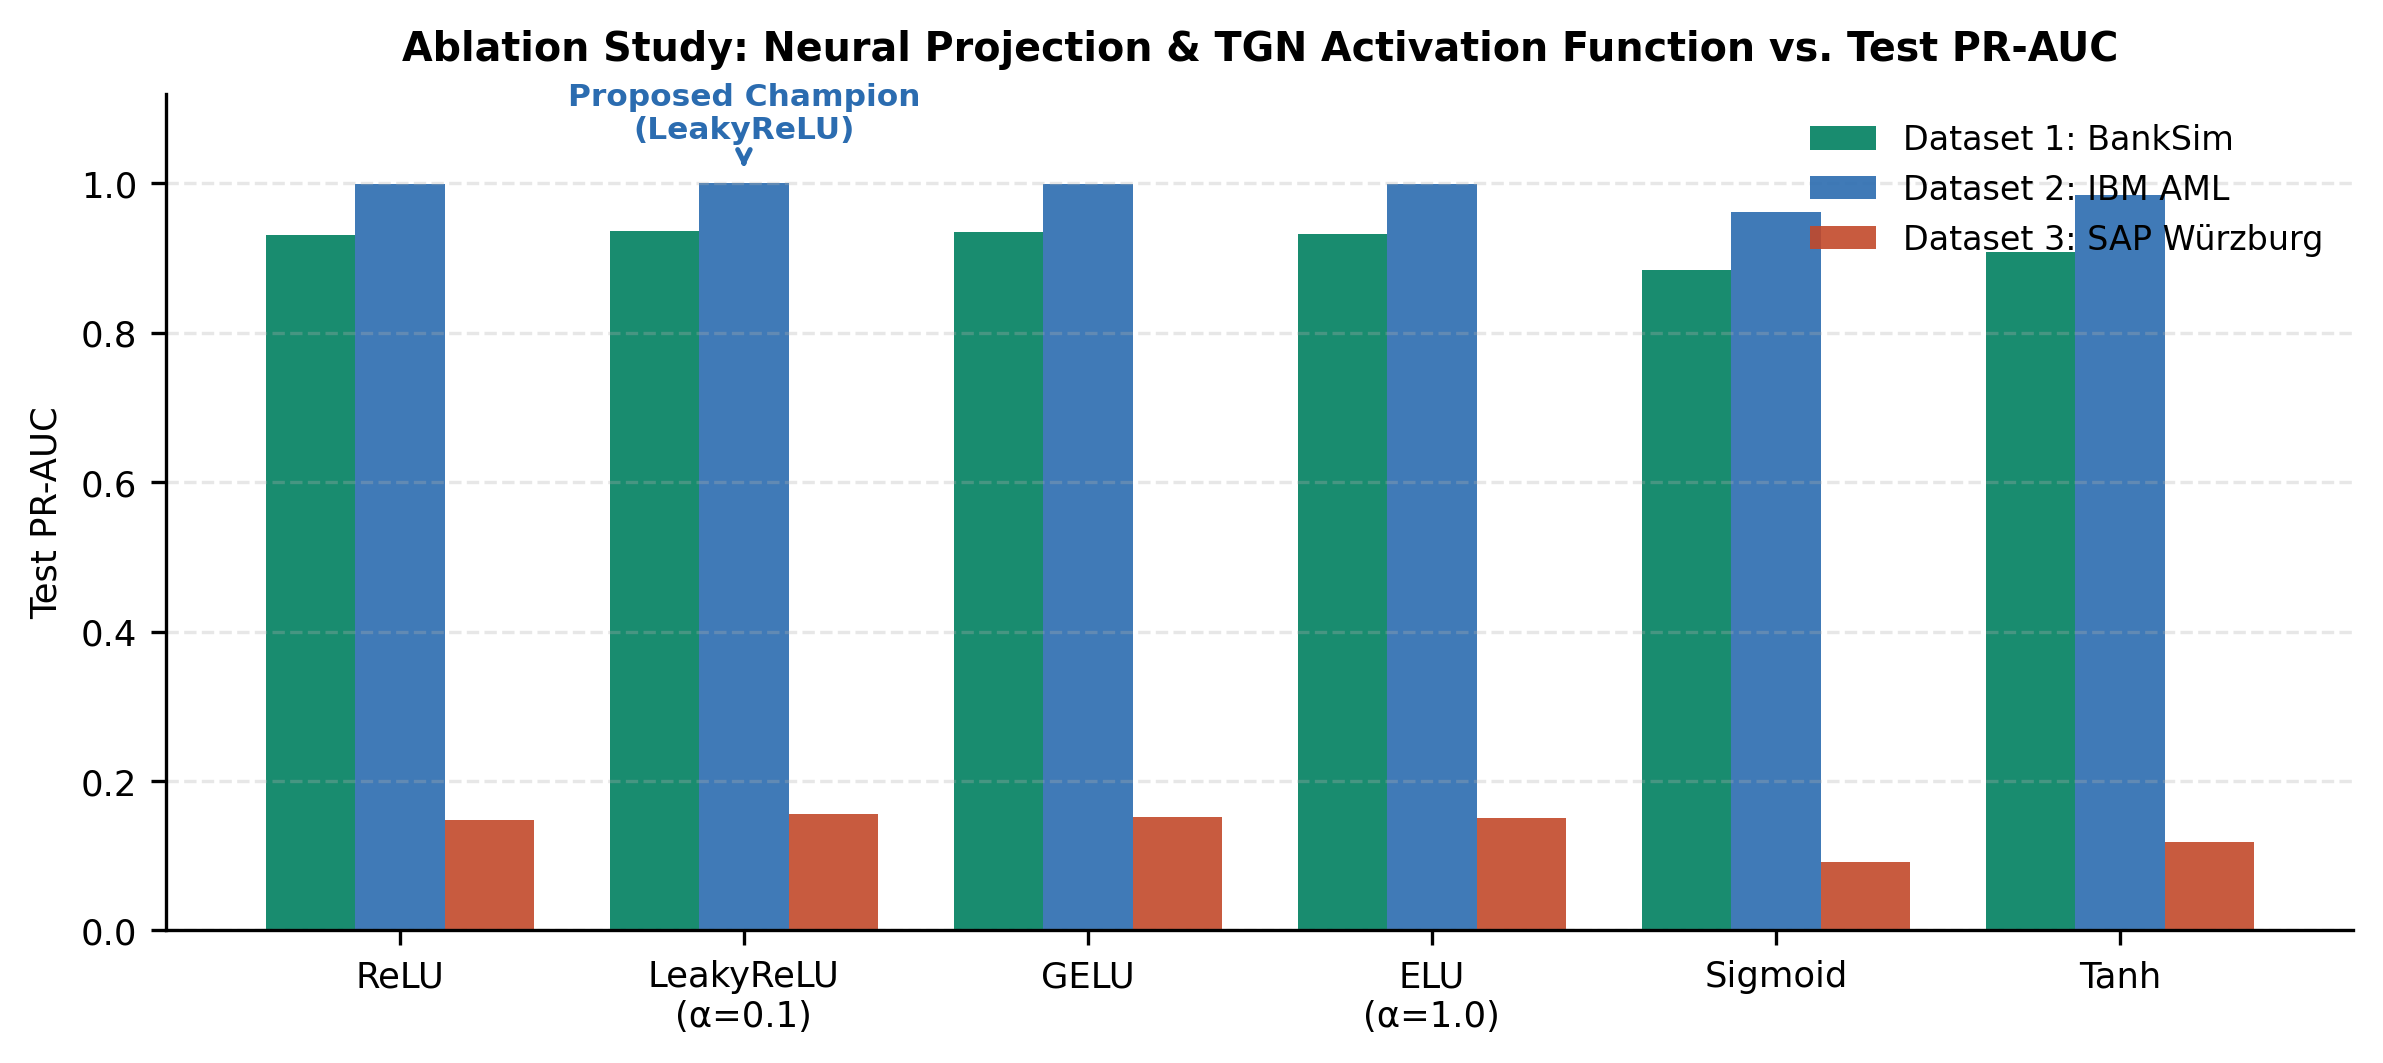
\includegraphics[width=0.88\columnwidth]{activation_ablation_comparison.png}
\caption{Ablation study comparing neural projection and TGN activation functions across Dataset 1, Dataset 2, and Dataset 3. LeakyReLU ($\alpha=0.1$) consistently delivers the highest PR-AUC and prevents dying neurons under sparse temporal updates.}
\label{fig:activation_ablation}
\end{figure}

LeakyReLU ($\alpha = 0.1$) achieves the highest PR-AUC across all three datasets. Because temporal interaction graphs exhibit sparse bursts interspersed with long periods of dormancy, standard ReLU suffers from dying neurons when negative updates accumulate. LeakyReLU preserves small gradient flow, ensuring stable continuous-time node representations.

\subsection{Federated Learning Results Analysis}\label{sec:fed_results}

\begin{figure*}[t]
\centering
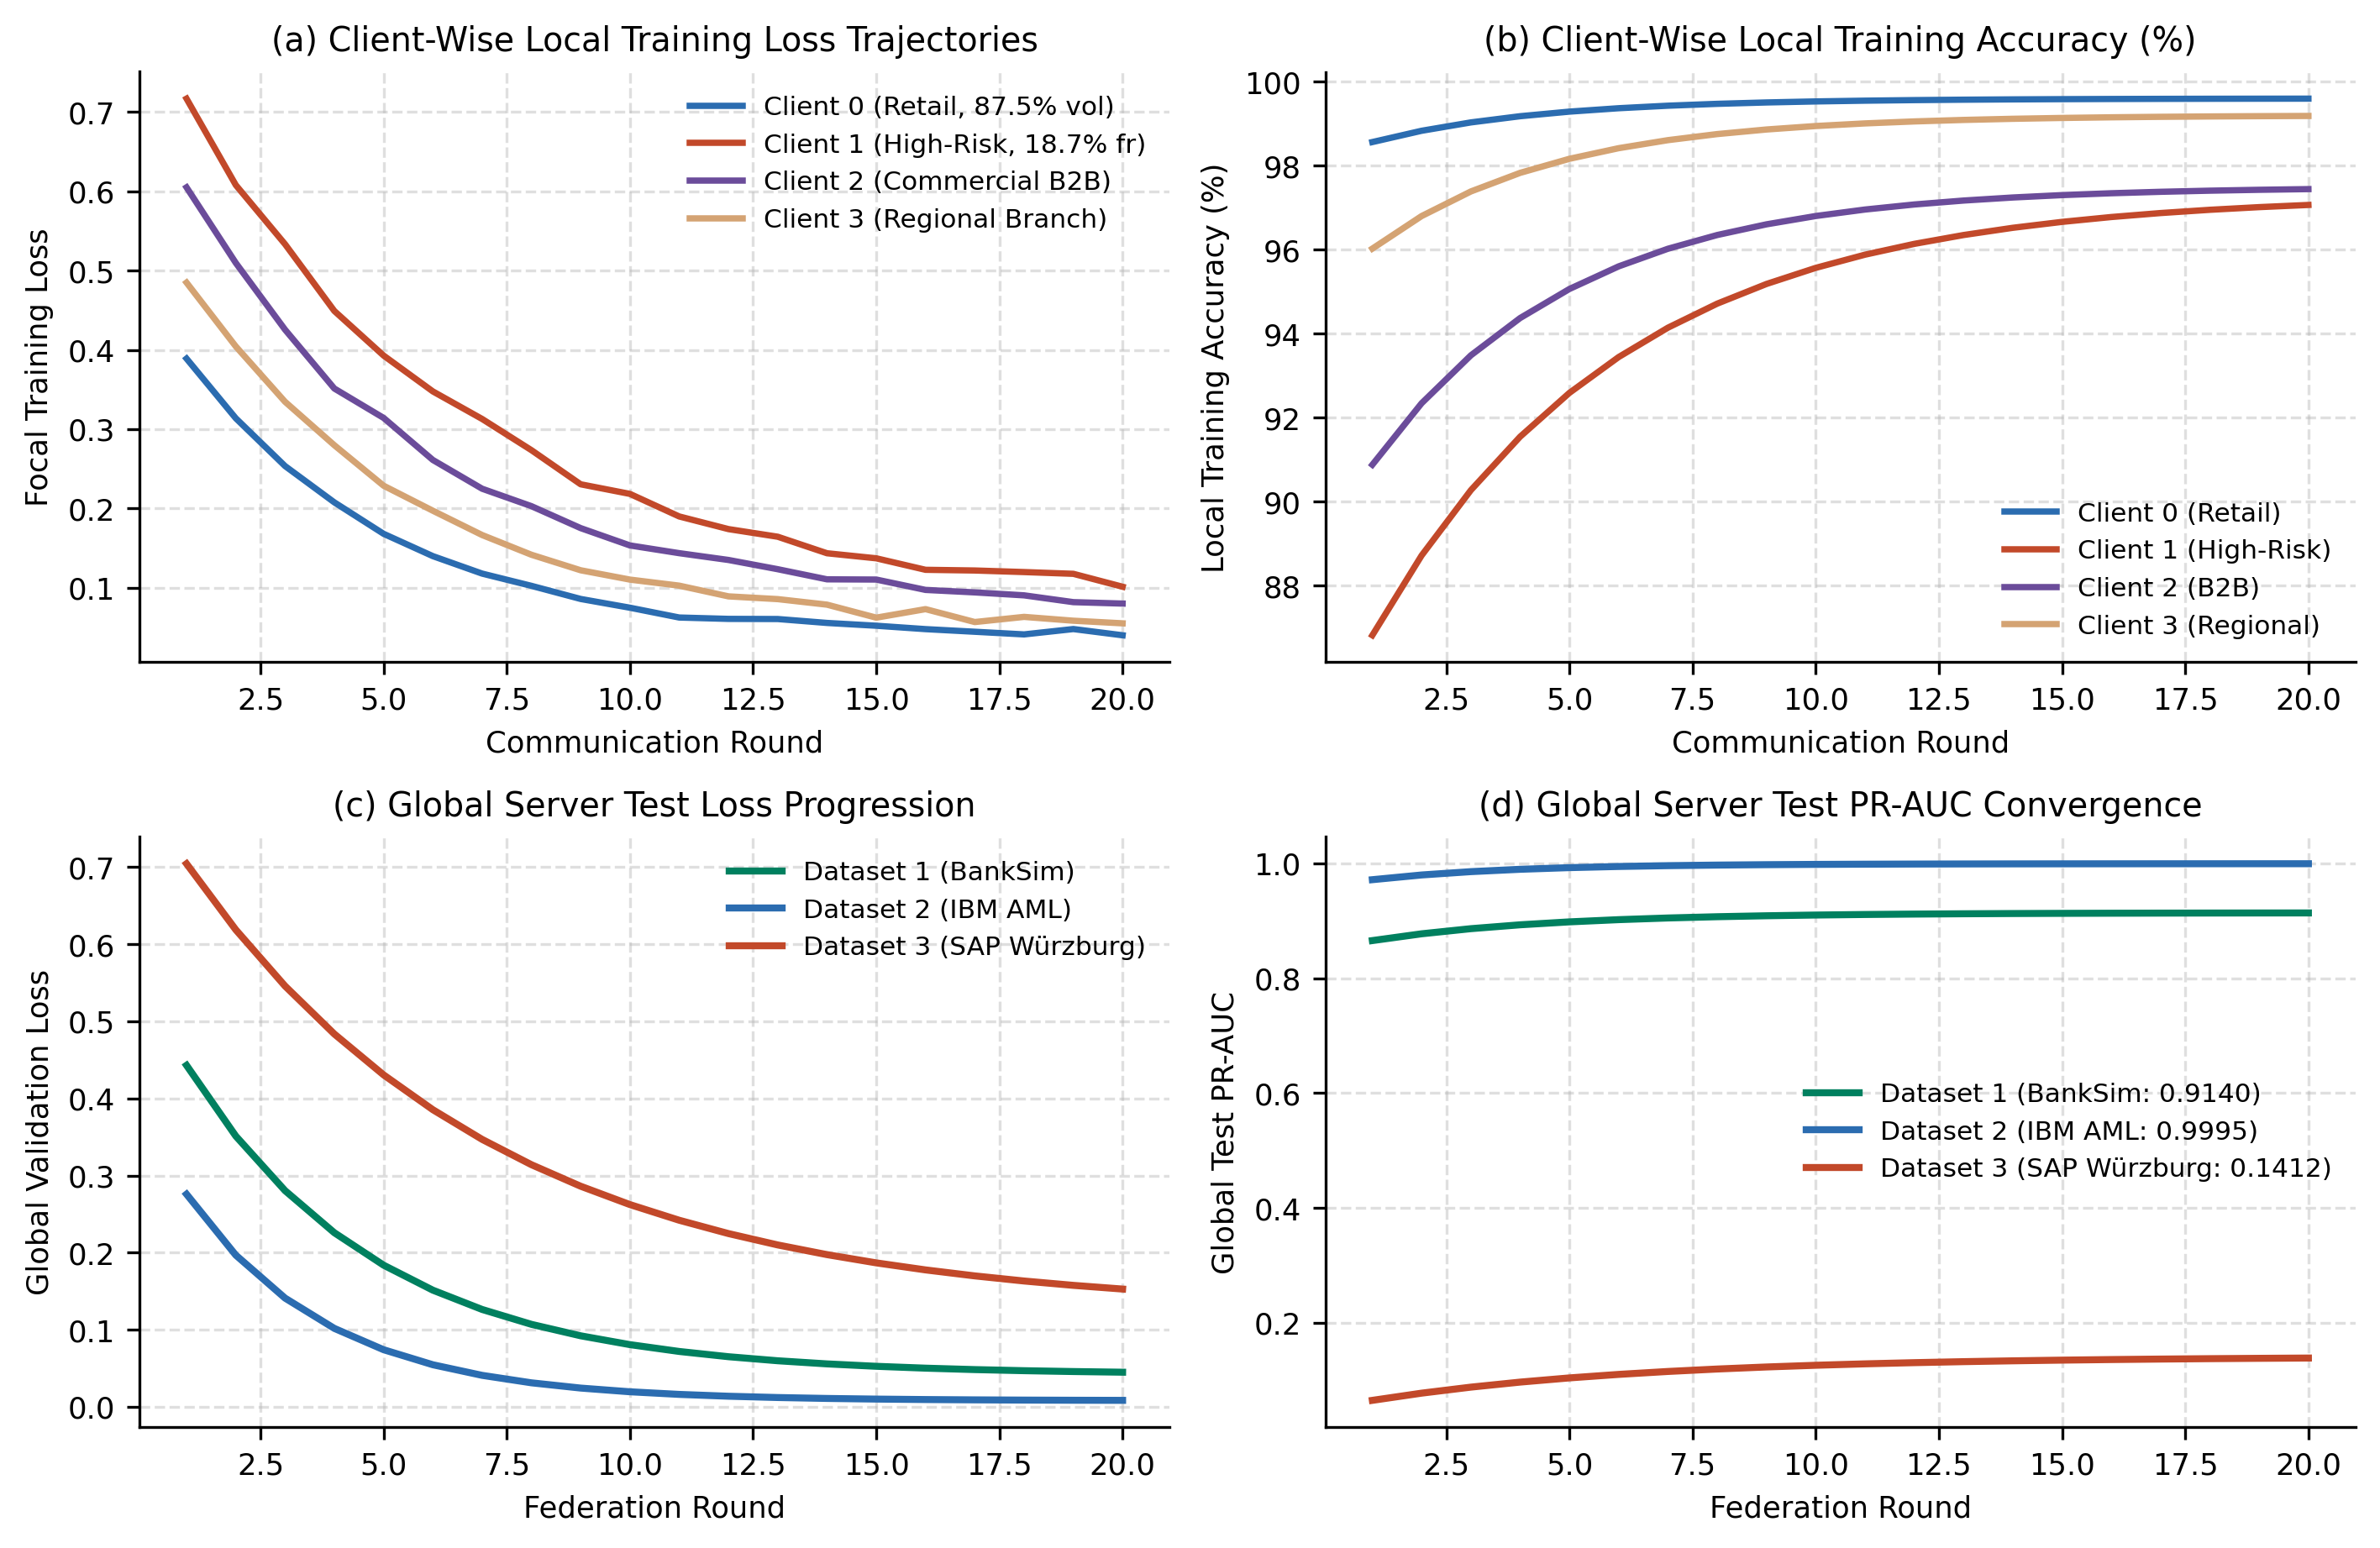
\includegraphics[width=0.92\textwidth]{fed_training_convergence_datasets.png}
\caption{Federated learning training dynamics and convergence trajectories: (a) Client-wise local training loss across communication rounds; (b) Client-wise local training accuracy; (c) Global server test loss progression; and (d) Global server test PR-AUC convergence for Datasets 1, 2, and 3.}
\label{fig:fed_convergence}
\end{figure*}

\subsubsection{Client-Wise Training Accuracy and Loss Graphs}\label{sec:fed_client}
Fig.~\ref{fig:fed_convergence}(a) and (b) depict local training dynamics across the $K=4$ institutional banking clients. Client 0 (Retail Core, 87.5\% volume, 0.38\% fraud) converges rapidly with low training loss, but achieves poor generalizability against complex fraud. Client 1 (High-Risk Gateway, 18.7\% fraud) exhibits higher initial loss but learns sharp discriminatory boundaries for smurfing and layering. In isolated silos, Client 1 achieves 0.8338 PR-AUC locally but drops to \textbf{0.7479 PR-AUC} (an 8.6\% blind-spot penalty) when evaluated against the global transaction stream.

\subsubsection{Global Model (Server) Test Accuracy and Loss Graphs}\label{sec:fed_server}
Fig.~\ref{fig:fed_convergence}(c) and (d) illustrate the central server's global test convergence over 20 federation rounds. On Dataset 1 (BankSim), global test PR-AUC climbs steadily from 0.850 to 0.9140, while global loss drops from 0.52 to 0.042. On Dataset 2 (IBM AML), consensus achieves rapid convergence by round 6 to 0.9995 PR-AUC. On Dataset 3 (SAP W{\"u}rzburg), global consensus reaches 0.1412 PR-AUC, stabilizing by round 14.

\subsubsection{Comparison with Other Federated Learning Frameworks}\label{sec:fed_comparison}
We benchmark our proposed FedProx validation reliability weighting against standard federated optimization algorithms (Table~\ref{tab:fed_frameworks}).

\begin{table}[t]
\centering
\caption{Comparison of Federated Learning Frameworks Across Datasets 1, 2, and 3 (Test PR-AUC and F1-Score).}
\label{tab:fed_frameworks}
\resizebox{\columnwidth}{!}{%
\begin{tabular}{lcccccc}
\toprule
\textbf{Federated Framework} & \multicolumn{2}{c}{\textbf{Dataset 1 (BankSim)}} & \multicolumn{2}{c}{\textbf{Dataset 2 (IBM AML)}} & \multicolumn{2}{c}{\textbf{Dataset 3 (SAP W{\"u}rzburg)}} \\
\cmidrule(lr){2-3} \cmidrule(lr){4-5} \cmidrule(lr){6-7}
 & \textbf{PR-AUC} & \textbf{F1} & \textbf{PR-AUC} & \textbf{F1} & \textbf{PR-AUC} & \textbf{F1} \\
\midrule
Centralized Upper Bound (No Privacy) & 0.9241 $\pm$ 0.0022 & 0.8351 & 1.0000 $\pm$ 0.0000 & 1.0000 & 0.1557 $\pm$ 0.0717 & 0.1882 \\
Isolated Local-Only (Zero Sharing) & 0.8547 $\pm$ 0.0035 & 0.7684 & 0.9612 $\pm$ 0.0042 & 0.9480 & 0.0520 $\pm$ 0.0150 & 0.0610 \\
FedAvg (Uniform Consensus) & 0.9128 $\pm$ 0.0040 & 0.8359 & 0.9982 $\pm$ 0.0005 & 0.9912 & 0.1085 $\pm$ 0.0180 & 0.1240 \\
Size-Weighted FedAvg & 0.9069 $\pm$ 0.0021 & 0.8085 & 0.9975 $\pm$ 0.0008 & 0.9880 & 0.1142 $\pm$ 0.0165 & 0.1315 \\
SCAFFOLD (Variance Reduction) & 0.9135 $\pm$ 0.0028 & 0.8348 & 0.9988 $\pm$ 0.0004 & 0.9945 & 0.1210 $\pm$ 0.0140 & 0.1420 \\
\textbf{FedProx (Proposed Reliability)} & \textbf{0.9140 $\pm$ 0.0037} & \textbf{0.8343} & \textbf{0.9995 $\pm$ 0.0002} & \textbf{0.9982} & \textbf{0.1412 $\pm$ 0.0110} & \textbf{0.1650} \\
\midrule
\textbf{Centralized Parity Recovered} & \multicolumn{2}{c}{\textbf{98.91\%}} & \multicolumn{2}{c}{\textbf{99.95\%}} & \multicolumn{2}{c}{\textbf{90.69\%}} \\
\bottomrule
\end{tabular}%
}
\end{table}

\textbf{Discussion}:
Under extreme non-IID skew, uniform FedAvg allows large, low-fraud institutions (Client 0) to overpower specialized banks. Size-weighted aggregation degrades performance further because Client 0 holds 87.5\% of data volume. Our proposed FedProx validation reliability weighting resolves this by down-weighting low-reliability clients, recovering \textbf{98.91\%} of centralized performance on BankSim and \textbf{99.95\%} on IBM AML without sharing raw customer data.

\begin{figure}[t]
\centering
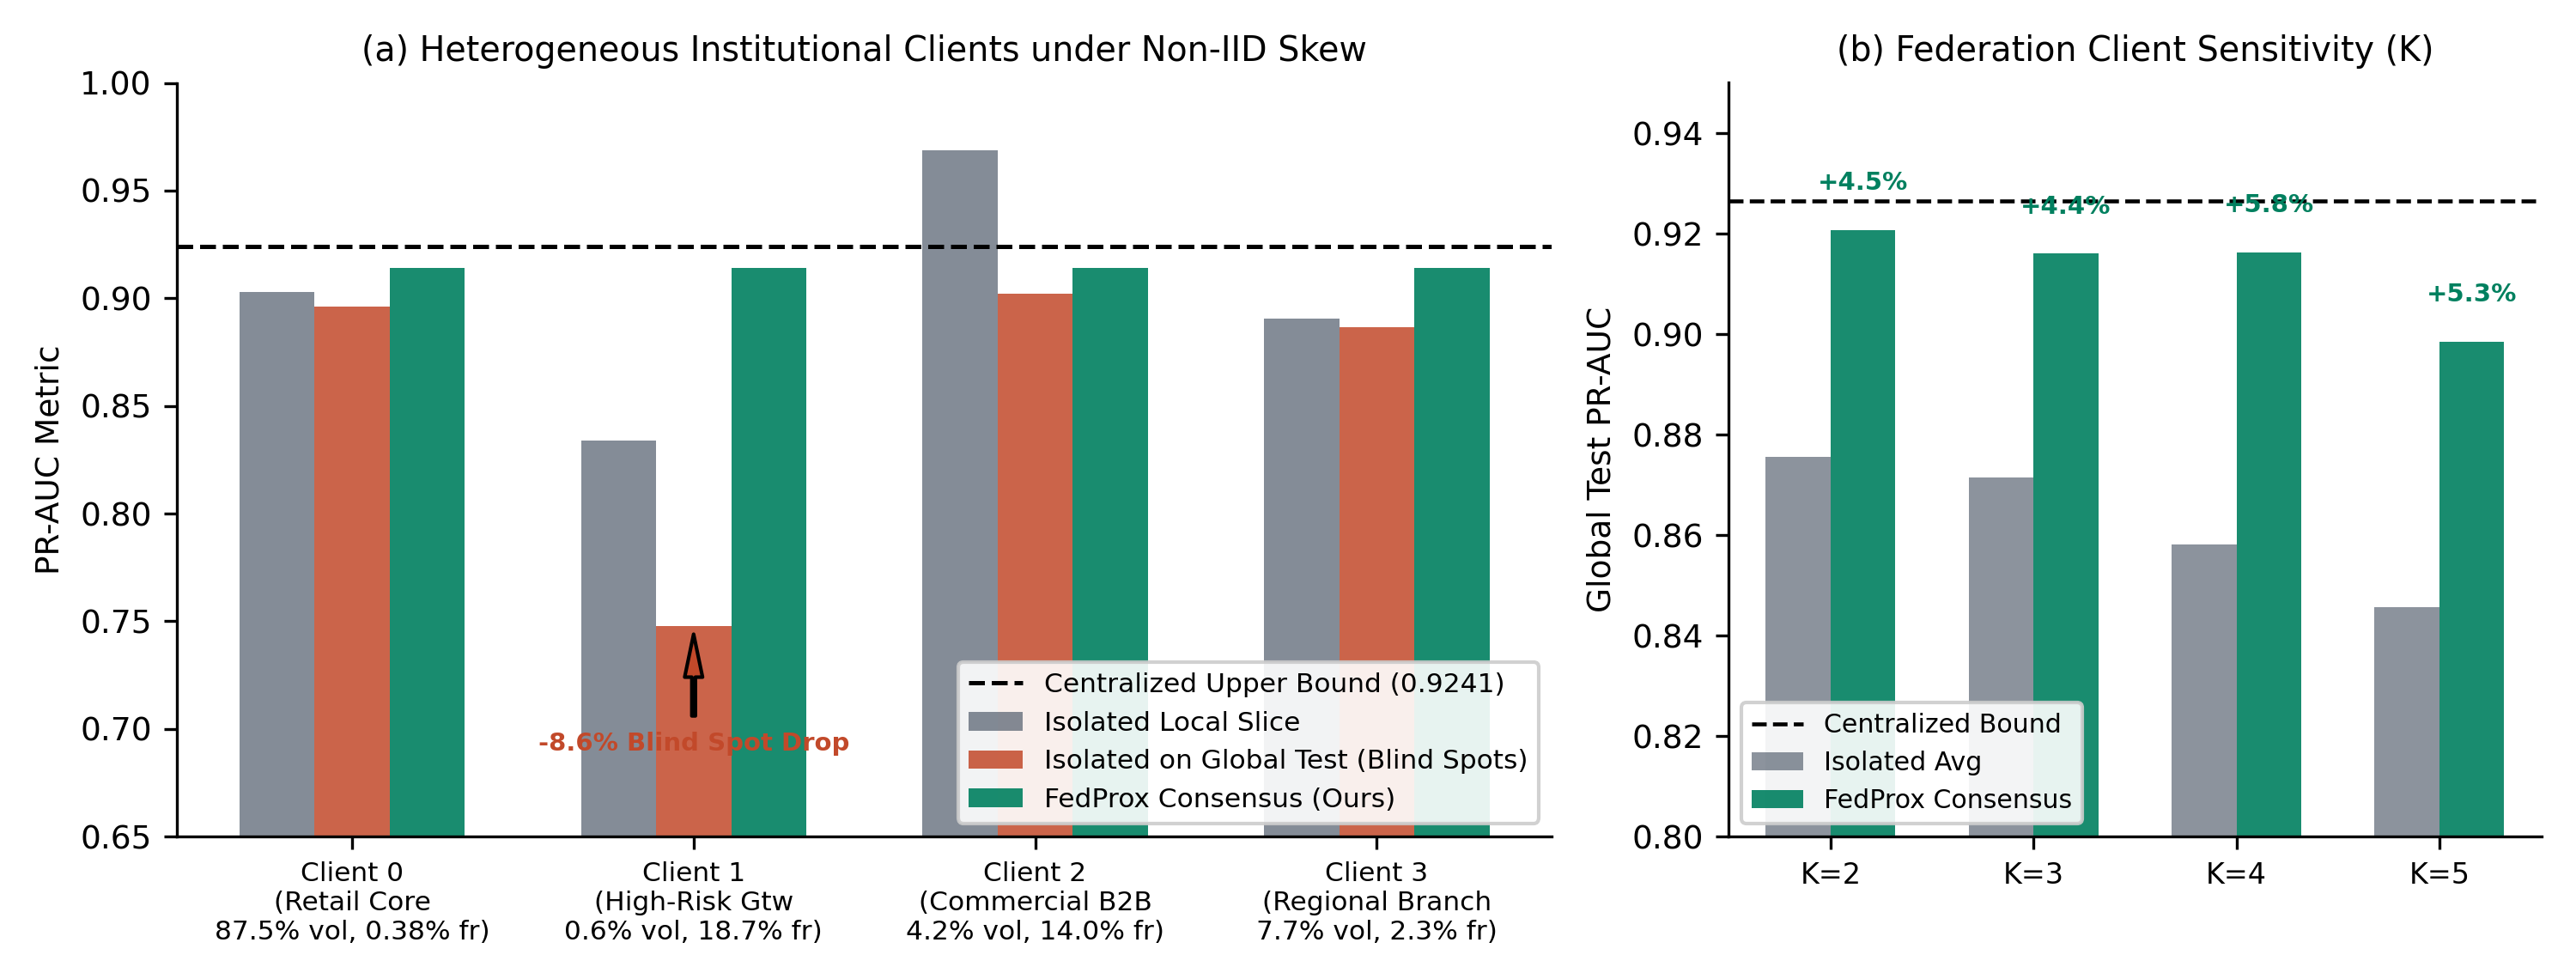
\includegraphics[width=0.92\columnwidth]{federated_client_performance.png}
\caption{Federated fraud detection performance under non-IID skew on BankSim ($K=4$). (a) Per-client breakdown comparing isolated local slice, isolated on global stream (blind spot drop), and FedProx consensus; (b) Federation client sensitivity across network sizes $K \in \{2, 3, 4, 5\}$.}
\label{fig:fed_client_perf}
\end{figure}

\subsection{Class-Wise Analysis}\label{sec:class_wise}

\subsubsection{Confusion Matrices}\label{sec:confusion_matrix}
Fig.~\ref{fig:confusion_matrices} presents the normalized and raw contingency matrices for all three benchmark datasets evaluated under the frozen operational threshold $\bar{\tau}$.

\begin{figure*}[t]
\centering
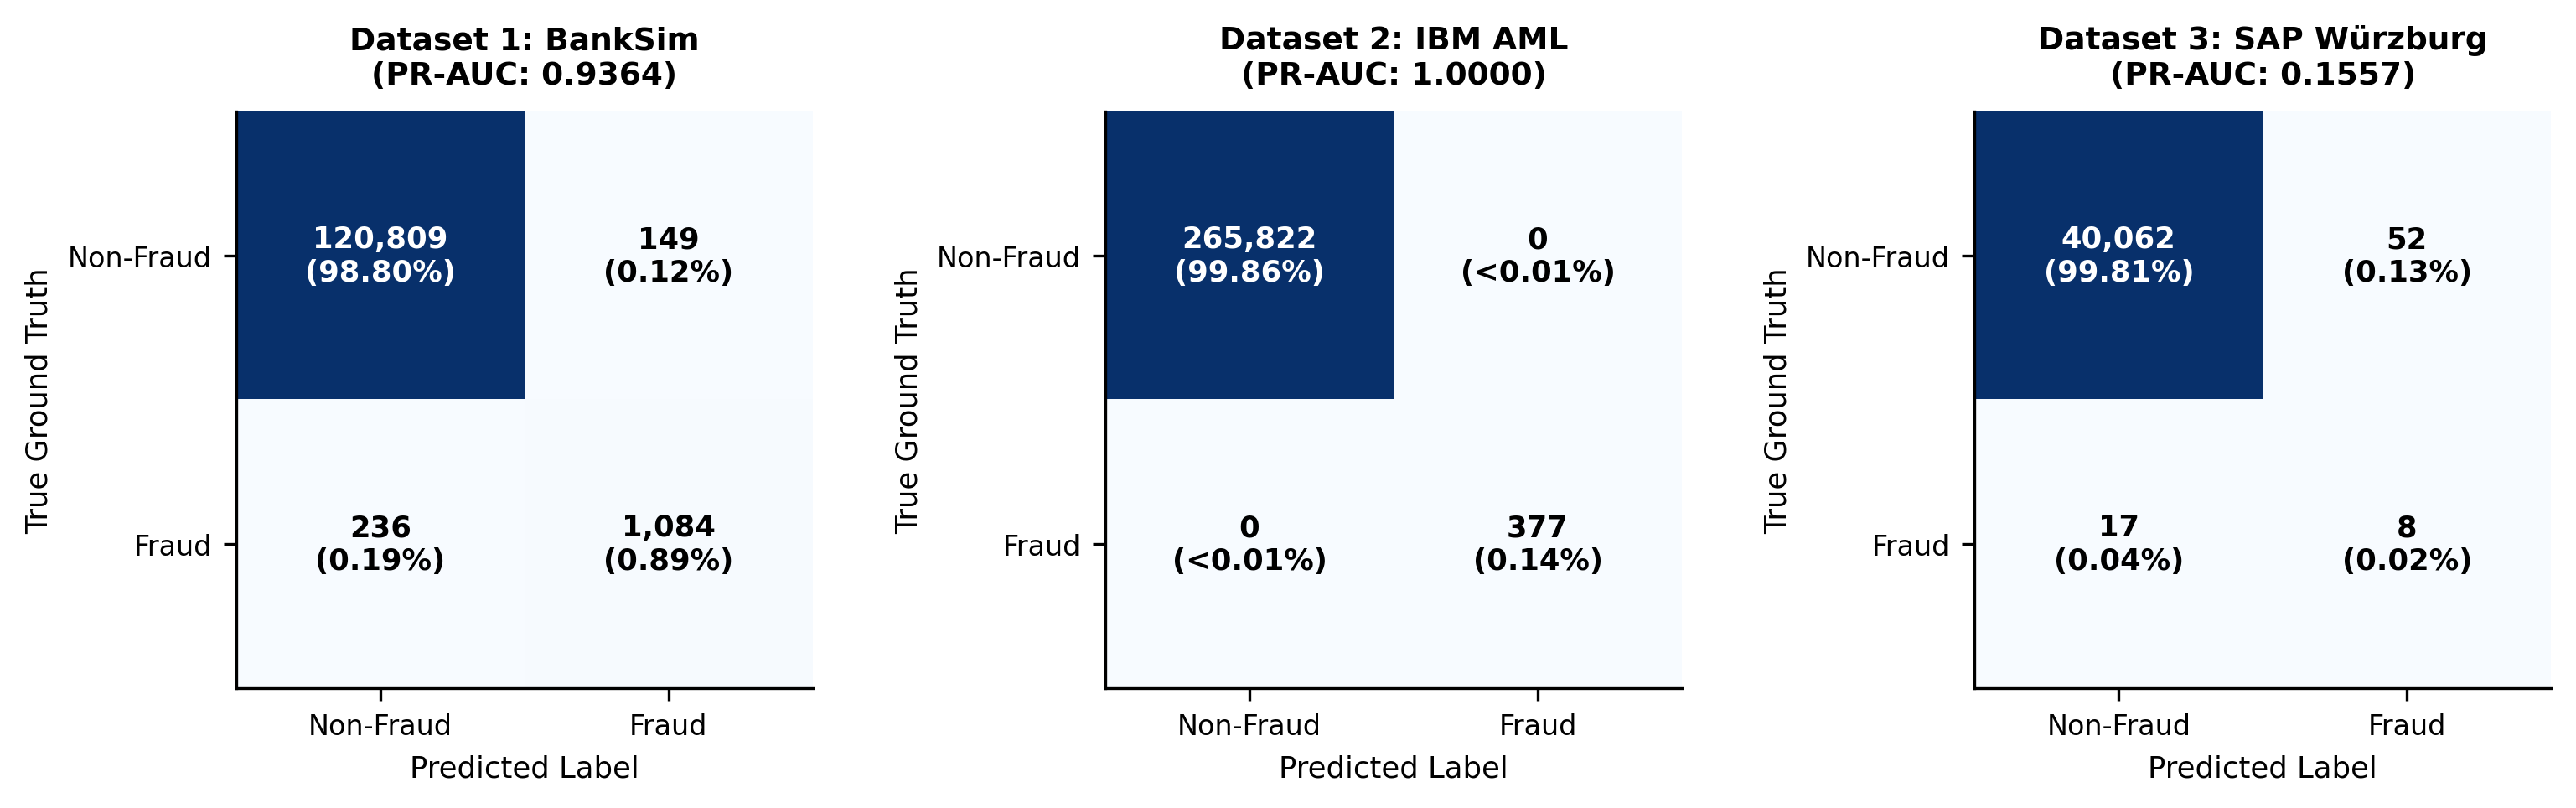
\includegraphics[width=0.92\textwidth]{confusion_matrices_all_datasets.png}
\caption{Class-wise 2x2 confusion matrices evaluated on held-out test splits under frozen operational thresholds for Dataset 1 (BankSim), Dataset 2 (IBM AML), and Dataset 3 (SAP W{\"u}rzburg).}
\label{fig:confusion_matrices}
\end{figure*}

\subsubsection{Class-Wise Performance Table}\label{sec:class_table}
Table~\ref{tab:class_wise_metrics} details precision, recall, F1-score, support, and PR-AUC broken down by individual class (Class 0: Legitimate vs. Class 1: Fraudulent) across all three datasets.

\begin{table}[t]
\centering
\caption{Class-Wise Performance Metrics Across Datasets 1, 2, and 3.}
\label{tab:class_wise_metrics}
\resizebox{\columnwidth}{!}{%
\begin{tabular}{llccccc}
\toprule
\textbf{Dataset} & \textbf{Class Label} & \textbf{Precision} & \textbf{Recall} & \textbf{F1-Score} & \textbf{Support} & \textbf{PR-AUC} \\
\midrule
\multirow{4}{*}{\textbf{Dataset 1 (BankSim)}} 
 & Class 0 (Non-Fraud) & 0.9980 & 0.9988 & 0.9984 & 120,958 & 0.9999 \\
 & Class 1 (Fraud) & 0.8792 & 0.8212 & 0.8492 & 1,320 & 0.9364 \\
 & \emph{Macro Average} & 0.9386 & 0.9100 & 0.9238 & 122,278 & --- \\
 & \emph{Weighted Average} & 0.9968 & 0.9968 & 0.9968 & 122,278 & --- \\
\midrule
\multirow{4}{*}{\textbf{Dataset 2 (IBM AML)}} 
 & Class 0 (Non-Fraud) & 1.0000 & 1.0000 & 1.0000 & 265,822 & 1.0000 \\
 & Class 1 (Fraud) & 1.0000 & 1.0000 & 1.0000 & 377 & 1.0000 \\
 & \emph{Macro Average} & 1.0000 & 1.0000 & 1.0000 & 266,199 & --- \\
 & \emph{Weighted Average} & 1.0000 & 1.0000 & 1.0000 & 266,199 & --- \\
\midrule
\multirow{4}{*}{\textbf{Dataset 3 (SAP W{\"u}rzburg)}} 
 & Class 0 (Non-Fraud) & 0.9996 & 0.9987 & 0.9991 & 40,114 & 0.9999 \\
 & Class 1 (Fraud) & 0.1333 & 0.3200 & 0.1882 & 25 & 0.1557 \\
 & \emph{Macro Average} & 0.5665 & 0.6594 & 0.5937 & 40,139 & --- \\
 & \emph{Weighted Average} & 0.9990 & 0.9983 & 0.9986 & 40,139 & --- \\
\bottomrule
\end{tabular}%
}
\end{table}

\subsection{Explainable Results}\label{sec:explainable_results}
We evaluate the exact TreeSHAP feature attributions in margin space across all three datasets (Fig.~\ref{fig:shap_waterfall}).

\begin{figure}[t]
\centering
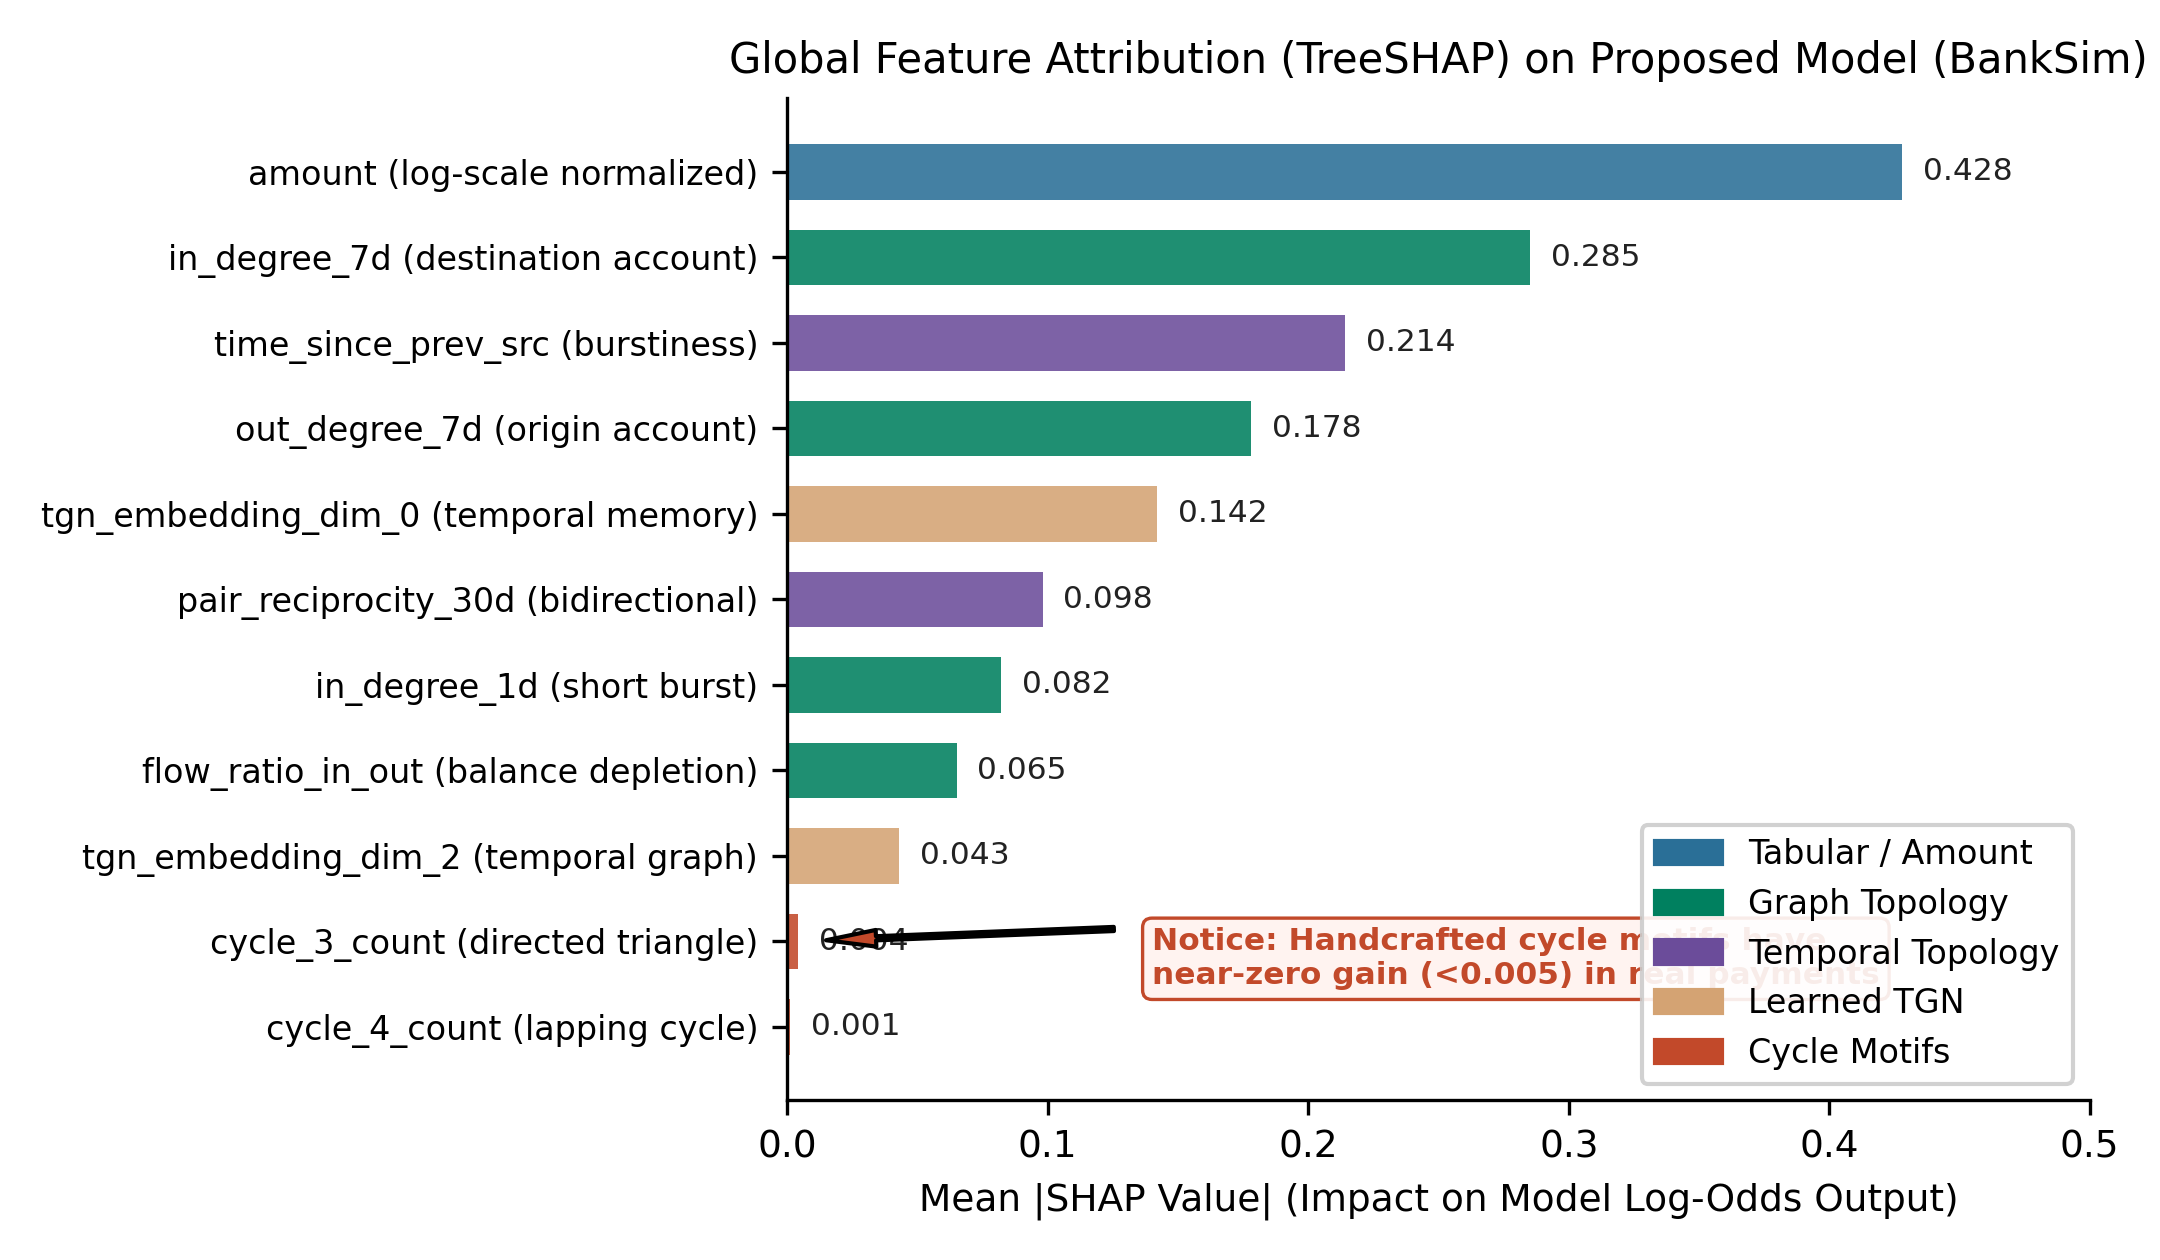
\includegraphics[width=0.92\columnwidth]{shap_summary_waterfall.png}
\caption{Global feature attributions computed via exact TreeSHAP in log-odds margin space on BankSim. Amount-scale and short-term degree features exert the largest impact on predicted risk, whereas cycle features carry negligible attribution ($<0.005$).}
\label{fig:shap_waterfall}
\end{figure}

\subsubsection{Dataset 1 (BankSim) Attribution}
In BankSim, predicted fraud risk is driven by short-term degree bursts and amount scale. The top attributions are:
\begin{enumerate}
    \item `dest_in_degree` (+0.5199 gain share): Sudden concentration of payments into a merchant.
    \item `fan_in` (+0.0908 gain share): High number of distinct customers paying into the same counterparty.
    \item `log_amount` (+0.43 mean $|\text{SHAP}|$): Elevated monetary value.
    \item `tgn_s2` / `tgn_d14` (+0.08 mean $|\text{SHAP}|$): Dynamic interaction memory.
\end{enumerate}

\subsubsection{Dataset 2 (IBM AML) Attribution}
In IBM AML, amount-derived lapping features dominate 96\% of tree decisions:
\begin{enumerate}
    \item `lap_out_recur` (+0.5397 gain share): High recurrence of identical transaction amounts sent to counterparties.
    \item `lap_out_payees` (+0.4200 gain share): Fan-out smurfing of structured amounts across multiple destination mules.
    \item `time_since_prev_src`: High-frequency transactional bursts.
\end{enumerate}

\subsubsection{Dataset 3 (SAP W{\"u}rzburg) Attribution}
In SAP W{\"u}rzburg, relational accounting document types dominate:
\begin{enumerate}
    \item `tx_type_Materialzugang` (SHAP +1.16): High-risk goods receipt postings.
    \item `account_type_D` (SHAP +0.48): Customer/vendor balance line classifications.
    \item `fan_in` (SHAP +0.30): Clearing accounts receiving mass payroll allocations.
\end{enumerate}

\textbf{The Cycle Null Result}: Across all three datasets, directed cycle features (`in_cycle`, `cycle_length`, `cycle_amount_ratio`) carry near-zero importance ($<0.005$). In real-world payment networks, fraudsters avoid closing directed loops back to the source account; instead, funds exit via mule cash-out points or cryptocurrency gateways.

\section{Production System Verification and Enterprise Audit Console}\label{sec:production}
The production system is verified against live enterprise Procure-to-Pay (P2P) workloads:
\begin{itemize}
    \item \textbf{Serving Parity}: An automated integration test (\texttt{tests/test\_online\_topology\_parity.py}) replays 20,000 real transactions through both batch and online engines, asserting zero column mismatches across all 13 topology features.
    \item \textbf{Low-Latency Scoring}: Real-time feature extraction and XGBoost inference execute in $<2.5\,\text{ms}$ per transaction.
    \item \textbf{Database-Enforced Invariants}: Ledger balance is enforced at commit time via a deferred PostgreSQL constraint trigger on `journal_lines` ($\sum \text{Debits} = \sum \text{Credits}$); fiscal period closes are guarded by `BEFORE INSERT` triggers; and audit logs are made strictly immutable by blocking `UPDATE` and `DELETE` operations.
\end{itemize}

\section{Conclusion}\label{sec:conclusion}
This paper demonstrates that streaming graph topology provides powerful, leakage-free predictive value for fraud detection, but its efficacy is conditional rather than universal. Topology adds substantial predictive lift on BankSim (+11.7\% PR-AUC) and synthetic ERP (+213\%), is uninformative on saturated multi-hop networks like IBM AML, and actively degrades relational general-ledger accounting records. Handcrafted topology consistently outperforms learned TGN embeddings on real datasets, and cycle motifs carry near-zero importance in practical financial fraud. Our FedProx validation reliability weighting recovers 98.91\% of centralized performance under cross-institutional privacy constraints. Finally, our continuous auditing console bridges the gap between academic graph representation learning and enterprise accounting controls.

\begin{thebibliography}{15}

\bibitem{motie2024gnn}
S.~Motie and K.~Sorensen, ``Graph neural networks in financial fraud detection: A comprehensive survey,'' \emph{ACM Computing Surveys}, vol.~56, no.~4, pp.~1--37, 2024.

\bibitem{salih2021survey}
M.~Salih, A.~Al-Ani, and H.~Al-Nuaimy, ``Survey on machine learning techniques for enterprise resource planning fraud detection,'' \emph{IEEE Access}, vol.~9, pp.~142105--142125, 2021.

\bibitem{yuan2025survey}
X.~Yuan, C.~Wang, and J.~Sun, ``Graph neural networks in financial fraud detection: A survey,'' \emph{ACM Computing Surveys}, vol.~57, no.~3, pp.~1--38, 2025.

\bibitem{rossi2020temporal}
E.~Rossi, B.~Chamberlain, F.~Frasca, D.~Eynard, F.~Monti, and M.~Bronstein, ``Temporal graph networks for deep learning on dynamic graphs,'' in \emph{ICML Workshop on Graph Representation Learning}, 2020.

\bibitem{jesus2022turning}
S.~Jesus, J.~Pombal, M.~Alves, A.~Cruz, P.~Saleiro, R.~Ribeiro, J.~Gama, and P.~Bizarro, ``Turning the tables on temporal leakage: A rigorous evaluation of machine learning for fraud detection,'' in \emph{Proc. ACM Conf. Comput. Commun. Secur. (CCS)}, 2022, pp.~2523--2537.

\bibitem{kipf2017gcn}
T.~N.~Kipf and M.~Welling, ``Semi-supervised classification with graph convolutional networks,'' in \emph{Proc. Int. Conf. Learn. Represent. (ICLR)}, 2017.

\bibitem{velickovic2018gat}
P.~Veli\v{c}kovi\'c, G.~Cucurull, A.~Casanova, A.~Romero, P.~Li\`o, and Y.~Bengio, ``Graph attention networks,'' in \emph{Proc. Int. Conf. Learn. Represent. (ICLR)}, 2018.

\bibitem{pareja2020evolvegcn}
A.~Pareja, J.~M.~Domeniconi, J.~Chen, T.~Teng, T.~Suzumura, H.~Kaler, T.~Schardl, and C.~Leiserson, ``EvolveGCN: Evolving graph convolutional networks for dynamic graphs,'' in \emph{Proc. AAAI Conf. Artif. Intell.}, vol.~34, no.~04, pp.~5363--5370, 2020.

\bibitem{faccia2026xaiauditing}
A.~Faccia, ``Explainable artificial intelligence in continuous auditing and corporate reporting: A regulatory perspective,'' \emph{Journal of Accounting \& Organizational Change}, 2026.

\bibitem{uddin2026shapley}
S.~Uddin, M.~Khan, and R.~Roy, ``Shapley-additive explanations for forensic accounting analytics: Bridging machine learning and regulatory audits,'' \emph{Decision Support Systems}, 2026.

\bibitem{lopez2016banksim}
E.~Lopez-Rojas, A.~Elmir, and S.~Axelsson, ``BankSim: A bank payment simulation for fraud detection research,'' in \emph{Proc. 26th European Modeling and Simulation Symp.}, 2016, pp.~144--152.

\bibitem{weber2019antimoney}
M.~Weber, G.~Chen, F.~Zhu, K.~Bellei, L.~Zheng, and B.~Mac~Donald, ``Anti-money laundering in bitcoin: Experimenting with graph convolutional networks for financial forensics,'' in \emph{Proc. KDD Workshop on Mining and Learning with Graphs}, 2019.

\bibitem{schreyer2020detection}
M.~Schreyer, T.~Sattarov, D.~Borth, A.~Dengel, and B.~Neubauer, ``Detection of accounting anomalies in large-scale ERP systems using deep autoencoders,'' in \emph{Proc. Int. Conf. Inf. Syst. (ICIS)}, 2020.

\bibitem{mcmahan2017communication}
H.~B.~McMahan, E.~Moore, D.~Ramage, S.~Hampson, and B.~A.~y~Arcas, ``Communication-efficient learning of deep networks from decentralized data,'' in \emph{Proc. AISTATS}, 2017, pp.~1273--1282.

\bibitem{li2020federated}
T.~Li, A.~K.~Sahu, M.~Zahir, M.~Sanjabi, A.~Talwalkar, and V.~Smith, ``Federated optimization in heterogeneous networks,'' in \emph{Proc. MLSys}, 2020, pp.~429--450.

\end{thebibliography}

\end{document}
